\documentclass[12pt,a4paper]{article}

% Engine-specific setup (for XeLaTeX or LuaLaTeX)
\usepackage{fontspec}
\setmainfont{MinionPro}
\setmathrm{Minion Pro}

% Geometry and layout
\usepackage[]{geometry}
\usepackage{setspace} 
\usepackage{fancyhdr}
\usepackage{lastpage}
\usepackage[absolute]{textpos}

% Encoding and language
\usepackage{graphicx}
\usepackage{xcolor}
\usepackage{url}
\usepackage{hyperref}
\usepackage{datetime}
\usepackage{amsmath, amsfonts, mathtools}
\usepackage{lscape}
\usepackage{wrapfig}
\usepackage{tikz}
\usepackage{epigraph}
\usepackage{tabto}
\usepackage{array}
\usepackage{booktabs}
\usepackage{longtable}
\usepackage{multirow}
\usepackage{enumitem}
\usepackage[titletoc,page]{appendix}
\usepackage{epstopdf}
\usepackage[acronym]{glossaries}
\usepackage{tcolorbox}
\usepackage{subfig} % Consider using subcaption for newer projects
\usepackage{csquotes}
\usepackage{algorithm}
\usepackage{algpseudocode}
\usepackage{rotating}
\usepackage{siunitx}
\usepackage{grffile}
\usepackage{tabularx}
\usepackage{pdfpages}

\onehalfspacing


% Bibliography
\usepackage[backend=biber, style=apa, sorting=anyt]{biblatex}
\addbibresource{bib.bib}



\title{From Barriers to Breakthrough: How Middle Management Shapes Sustainable Innovation in Disruptive Industries}
\author{Shruti Dubey}
\date{June, 2025}




\begin{document}
	
	\hypersetup{
		colorlinks=false,
		linkbordercolor=white,
		linkcolor=white,
		filecolor=white,      
		urlcolor=white,
		citecolor=white,
	}
	

	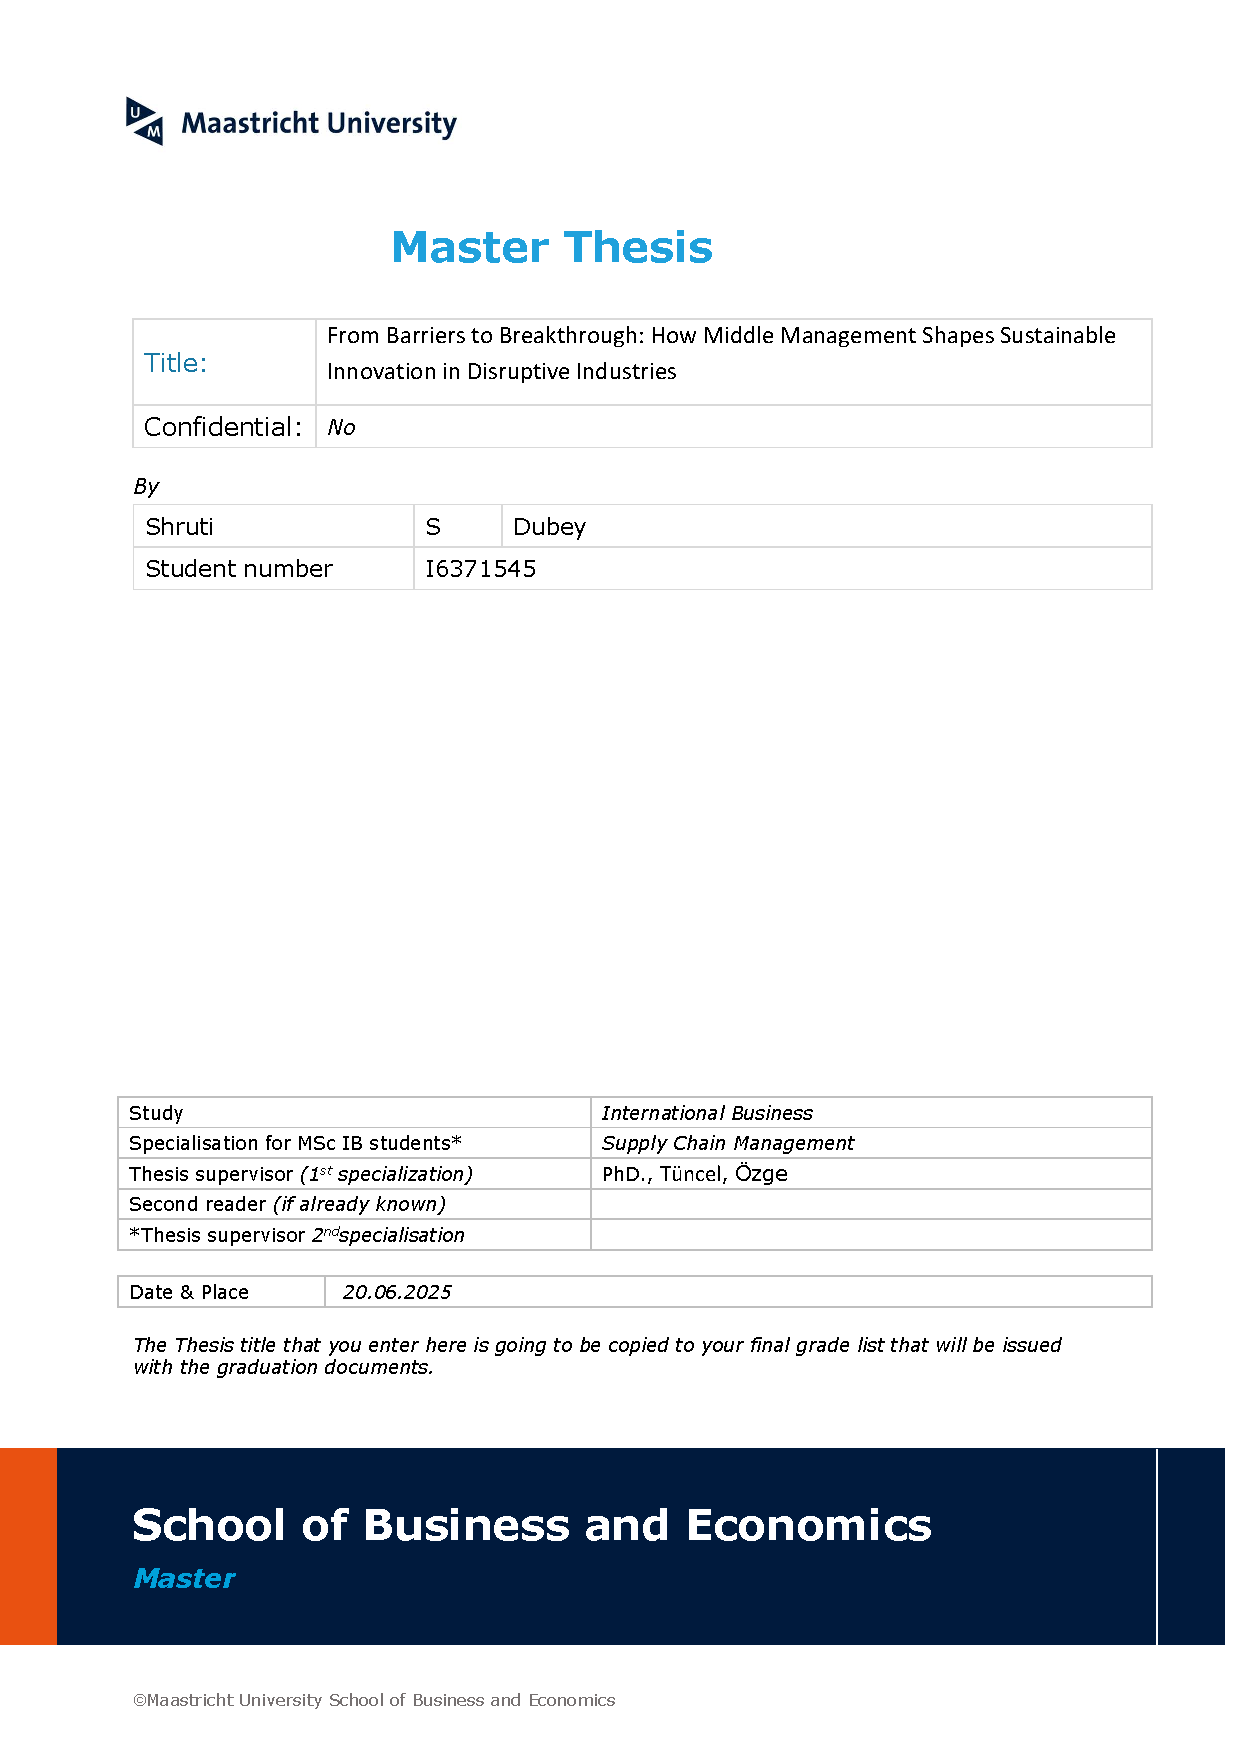
\includepdf[pages=-]{Images/MainPage.pdf}
	
\begin{center}
	\section*{Acknowledgements}
\end{center}
	I would like to express my deepest gratitude to my supervisor, Dr Özge Tüncel, for her invaluable guidance and support throughout every stage of this research. I am also sincerely thankful to the managers from the clean energy and cultured meat sectors who generously shared their time and insights during interviews, making this study possible. My heartfelt appreciation to my friends and family; especially my mom; for their understanding and encouragement during this journey. Most of all, I am overwhelmingly grateful to my partner Mohit, whose love, patience, support, and belief in me have been a continual source of strength. Thank you for your presence, it has made every challenge lighter and every success more meaningful.
	\newpage
\begin{center}
	\section*{Abstract}
\end{center}
		This thesis investigates how middle management drives sustainable innovation in disruptive industries, focusing on clean energy and cultured meat. Through qualitative interviews with managers from both sectors, the study compares strategies for overcoming technical, regulatory, and market barriers. Findings reveal that clean energy managers prioritize process optimization, regulatory compliance, and stakeholder partnerships, while cultured meat managers emphasize regulatory adaption, consumer education, and innovation. Across both sectors, effective communication, internal alignments, and external collaboration are key to progressing sustainability. The research extends sustainability leadership theory beyond executive roles, offering practical frameworks for endowing middle managers and accelerating sustainability transitions in emerging industries.

	\newpage
	\tableofcontents
	\newpage
	\listoftables
	\listoffigures
	\newpage
	
    
\section{Introduction}

Increasing global demand for sustainable development has transformed industrial approaches. Disruptive sectors like clean energy and cultured meat are growing, driving innovation and new business models (\textcite{SeedBlink2025, Deloitte2025}). Disruptive technologies transform existing markets and business models by introducing new value propositions, replacing existing products, services, or manufacturing processes (\textcite{Bower1995}). Among these emerging sectors, cultured meat and clean energy solutions are increasingly recognized for their potential to address critical challenges such as climate change, resource shortages, and food security (\textcite{Wageningen2022, GFI2025future}). For example, global renewable capacity increased by 50\% from 2022 to 2023, with solar PV and wind accounting for a record 96\% of that growth. This highlights solar energy?s primary role in decarbonization. Similarly, research on cultured meat shows it could significantly minimize land use, greenhouse gas emissions, antibiotic use, and animal welfare impacts compared to conventional meat. This industry is rapidly expanding, with over 170 companies emerging by 2023 and securing billions in funding based on environmental and ethical claims.

\paragraph*{} Despite these promises, most research examines technological and market aspects while neglecting lower and middle management considerations.

\paragraph*{}
Literature on solar energy extensively examines technical innovations like grid integration and energy storage (\textcite{SINSEL20202271}). Similarly, existing research in cultured meat focuses on production processes and regulatory pathways (\textcite{Bryant2020}). While these sectors offer revolutionary environmental and economic benefits, their widespread adoption and scaling are limited by technical, organizational, and systemic barriers that vary across industries. These examples show that promising green industries are often operationally complex, facing challenges ranging from finance and supply chain logistics to consumer education and regulatory compliance.

\paragraph*{} While management commitment is acknowledged as vital for sustainability in disruptive industries, comparative, sector specific research is lacking to examine how on middle management navigates unique barriers and leverage enablers across different disruptive contexts (\textcite{Lozano2015, Egri2000}).

\paragraph*{} Addressing this research gap is crucial for the tangible benefits these comparative insights can offer. This study's focus on middle management within the disruptive contexts of clean energy and cultured meat offers substantial theoretical and practical contributions. Theoretically, by examining middle management?s role in these novel disruptive contexts, this research seeks to extend theories of sustainable leadership, which have predominantly focused on executive roles, and offer a more granular understanding of how strategy is operationalized in environments characterized by high uncertainty and rapid innovation.

\paragraph*{} Practically, comparative insights aim to provide actionable strategies for middle managers to more effectively navigate common and sector specific barriers related to technology development, market acceptance, and resource allocation, thereby potentially accelerating sustainability transitions in their respective fields. These insights may also inform policy design and investment strategies aimed at supporting these vital industries. A nuanced understanding of how middle managers enact sustainability in practice can help organizations in these rapidly evolving sectors to better harness their innovative capacity, overcome critical adoption hurdles, and ultimately enhance their contribution to global sustainability goals such as climate change mitigation and food security.

\paragraph*{} Furthermore, the comparative element in this research is central to achieving these contributions. By placing the developing cultured meat sector with the evolving clean energy industry, this study aims to pinpoint how middle managers drive sustainability. It identifies both industry specific strategies and universal best practices, contributing to developing more robust managerial frameworks for sustainable innovation.

		\section{Literature Review}
	\label{sec:litreview}
	
	Building on the introduction, which outlined the rising significance of sustainable innovation in disruptive industries such as clean energy and cultured meat, this literature review critically examines the current state of academic and industry knowledge on how sustainability is managed and implemented within these emerging sectors. While sustainability and disruption are widely discussed in management literature, most analyses remain concentrated at the level of technological feasibility or executive decision making. There is limited understanding of how sustainability is translated into practice within organizations, especially by middle managers who bridge strategic directives and day-to-day operations. This oversight is particularly problematic given that middle managers serve as crucial intermediaries between strategic vision and operational execution, yet their specific role in sustainable innovation within disruptive contexts remains largely unexplored \cite{Floyd1997}. While these industries offer significant potential for addressing global sustainability challenges, their success depends critically on effective management practices that can navigate high uncertainty and rapid change \cite{Christensen1997}. \\
	
	This literature review examines the intersection of management practices and sustainable innovation in disruptive industries, with particular focus on identifying the research gap concerning middle management’s role. By analyzing the distinct challenges within cultured meat and renewable energy sectors, this review establishes the theoretical foundation for understanding how middle managers contribute to sustainability transitions in rapidly evolving industries. \\
	
	\subsection*{Structure of the Literature Review}
	This literature review examines seven key themes that collectively build the case for studying middle management in sustainable innovation. First, it establishes management’s fundamental role in driving sustainability outcomes. Second, it highlights the current research emphasis on executive leadership. Third, it examines why generic sustainability frameworks may be insufficient for disruptive industries. Fourth, it defines disruption within sustainable innovation contexts. Fifth, it analyzes specific barriers in cultured meat and renewable energy sectors. Sixth, it explores market adoption challenges in translating innovation to impact. Finally, it identifies the research gap regarding middle management’s role in sustainability transitions. Each section synthesizes academic literature and industry evidence to support the need for focused research on middle management in disruptive sustainable industries. \\
	
	\subsection{The Strategic Role of Management in Corporate Sustainability}
	The integration of sustainability into corporate strategy is increasingly recognized as a cornerstone of long-term organizational success. A growing body of literature emphasizes the critical role of management, particularly top executives, in embedding sustainability principles within business operations. Leadership commitment at the highest levels acts as a catalyst for systemic change, setting the tone for sustainable practices across the organization \textcite{Avery2005}, \textcite{Waldman2008}. Sustainable leadership entails balancing economic, social, and environmental objectives through comprehensive and adaptive decision-making frameworks \cite{Lozano2015}. \\
	
	Eccles, Ioannou, and Serafeim (2014) provide empirical evidence through a longitudinal study of “High Sustainability” firms, demonstrating that companies with formal sustainability governance structures such as board-level oversight and executive incentive mechanisms outperform their peers financially over time \cite{Eccles2014}. These findings support the argument that top management is not merely a facilitator but a key enabler of effective and enduring sustainability transitions. \\
	
	The scope of managerial influence extends well beyond operational efficiency to encompass the cultivation of an organizational identity rooted in sustainability values. This transformation involves guiding strategic direction, enhancing stakeholder trust and legitimacy, and embedding sustainability principles into corporate DNA \cite{Eccles2014, Dyllick2016}. However, successful sustainability integration requires active participation across all hierarchical levels and stakeholder groups, including boards of directors, shareholders, and employees \cite{Freeman1984}. \\
	
	Recent studies on small and medium-sized enterprises (SMEs) and startups provide particularly compelling evidence of management’s mediating role in sustainability outcomes. Madrid-Gujjaro \& Duréndez (2023) and Memon et al. (2022) demonstrate how management commitment serves as a crucial bridge between sustainability drivers and environmental performance \cite{Madrid2023, Memon2022}. When top executives champion environmental values, firms demonstrate a significantly higher likelihood of implementing sustainable practices. \\
	
	In sum, the role of management spanning strategic vision, operational execution, and cultural transformation is indispensable in advancing corporate sustainability agendas and achieving enduring competitive advantage.
	
	\subsection{The Executive-Centric Focus and Its Limitations}
	Despite widespread recognition of management’s importance in sustainability, academic research exhibits a pronounced executive-centric bias that limits our understanding of sustainability implementation across organizational levels. The literature predominantly examines senior managers, CEOs, and boards of directors who set strategic direction and initiate sustainability initiatives, while systematically overlooking contributions from middle and lower management levels. \\
	
	This executive focus has established a prevailing narrative rooted in top-down leadership models. Upper Echelons Theory (UET) has gained prominence in sustainability research, explaining how top managers’ demographic, cognitive, and experiential characteristics—including age, tenure, education, and value orientation—influence corporate social responsibility (CSR) and sustainable innovation outcomes \cite{Waldman2008, Ioannou2015}. Researchers emphasize how top management teams shape organizational culture, allocate sustainability resources, and foster cross-sector collaboration, particularly when leaders adopt systems thinking approaches \cite{Dyllick2016}. \\
	
	Keil et al. (2024) exemplify this trend by identifying institutionalized sustainability responsibilities such as board-level oversight and formal top-down governance structures as among the strongest predictors of successful sustainability practices \cite{keil2024c}. Similarly, research on SMEs consistently highlights the central role of owner-managers in driving environmental performance \cite{kutzschbach2021c}, while studies of larger corporations focus on how executive compensation tied to environmental metrics drives superior financial and environmental performance \cite{Eccles2014}. \\
	
	However, this executive-centric perspective creates a substantial gap in understanding how sustainability strategies are operationalized. Middle managers translate strategic sustainability goals into practical actions. They coordinate cross-functional teams, allocate operational resources, and manage emergent challenges during implementation. Omitting middle management from academic discourse limits comprehension of how organizations embed sustainability in everyday practices and across hierarchical layers. \\
	
	This limitation becomes particularly problematic when examining SMEs, where organizational structures tend to be flatter and distributed leadership more common. Even in these contexts, research frequently attributes sustainability outcomes solely to top executives, obscuring the grassroots engagement and distributed leadership that drive sustainability implementation \cite{birkinshaw2010}. \\
	
	\subsection{Generalized Frameworks and Theoretical Limitations}
	A recurring limitation in the current sustainability literature is the tendency to rely on broad, generalized theoretical models that lack contextual specificity. Frameworks such as the triple bottom line and stakeholder theory are commonly applied due to their wide applicability, but their utility diminishes in specific or emerging industry settings. While these models offer valuable conceptual guidance, they often fail to capture the complexities of specific organizational contexts. Kutzschbach et al. (2021) argue that theories derived from large corporate environments do not easily translate to smaller firms or disruptive sectors, noting that “no coherent theory exists about the drivers of corporate sustainability in SMEs” \cite{kutzschbach2021a}. Similarly, Keil et al. (2024) observe that critical variables such as leadership behaviours, organizational culture, and employee engagement are frequently studied in isolation, resulting in fragmented insights rather than an integrated understanding of sustainable performance \cite{keil2024a}. \\
	
	This theoretical generality extends to empirical research, which emphasizes macro-level factors like national policies and technological innovations while overlooking organizational implementation processes. Studies on renewable energy focus on grid infrastructure and regulatory mechanisms, neglecting managers’ day-to-day operational practices \cite{IRENA2020}. Similarly, cultured meat research prioritizes technical processes and regulatory hurdles over leadership dynamics and managerial roles \cite{Bryant2020}. This creates a critical blind spot in understanding how sustainability strategies are operationalized at various managerial levels, particularly middle management, which bridges executive strategy and frontline implementation. \\
	
	\subsection{Conceptualizing Disruptive Industries in Sustainability Literature}
	Disruptive industries are characterized by technological or business model innovations that fundamentally alter existing markets and value networks. These include sectors such as renewable energy, cultured meat, and synthetic biology. Classic definitions of disruptive innovation, such as those by Tushman and Anderson (1986), emphasize technological discontinuities i.e. radical shifts in products, processes, or value chains \cite{Tushman1986}. More recent perspectives highlight the importance of scalable, novel approaches that replace traditional industry models \cite{Yu2010}. In business theory, disruptive innovation refers to innovations that begin by serving overlooked or underserved market segments with simpler, more affordable, and accessible offerings, and eventually displace established market leaders and their sustaining innovations \cite{Christensen1997}. These innovations often originate from startups or peripheral market players rather than incumbents, and their initial market appeal may not generate sufficient profit to attract attention from larger firms. Over time, however, they reshape the competitive landscape by targeting non-consumers or overserved customers with “good enough” solutions. \\
	
	The success of disruptive innovations depends not only on technology but on developing business models capable of redefining value delivery \cite{Chesbrough2007}. This highlights that effective management in disruptive industries requires a strategic orientation toward adaptability, innovation, and foresight beyond technical proficiency. However, disruptive sectors introduce unique challenges including regulatory uncertainty, consumer skepticism, and high capital intensity, which remain underexplored in sustainability research \cite{Wustenhagen2007}. \\
	
	The transformational nature of disruptive sectors implies that traditional management approaches may be inadequate. Managers must innovate at both technology and business model levels, proactively monitoring emerging trends, responding to market signals, and cultivating novel approaches to customer value creation under rapid change and uncertainty \cite{Teece2007}.\\
	
	\subsection{Barriers to Sustainability in Cultured Meat and Clean Energy}
	Cultured meat and clean energy industries both aim to advance sustainability but face markedly different types of barriers, reflecting their relative levels of maturity and technological pathways. Understanding these differences is crucial to assessing how middle managers operate within them. \\
	
	\subsubsection{Cultured Meat}
	The cultured meat industry presents significant potential for sustainable food systems by reducing reliance on conventional animal agriculture. However, it faces substantial technological, economic, and social barriers to scale and adoption. Technologically, the industry remains dependent on high energy input and growth media derived from animal serum or synthetic compounds, which undermines sustainability claims \cite{Specht2023, Post2020}. Additionally, cost-effective scalability remains elusive due to inefficient bioreactor designs, high input costs, and the lack of commercially viable scaffolds for structured meat production \cite{Bodiou2020}. Other unresolved technical challenges include replicating the nutritional profile of conventional meat and mitigating contamination risks in large-scale operations. \\
	
	From an economic standpoint, high production costs and capital-intensive processes limit commercial viability. Infrastructure remains nascent, and supply chains for bioreactors, culture media, and skilled labor are underdeveloped \cite{Stephens2018}. Social and ethical dimensions also pose challenges. Concerns about unnaturalness, food safety, and religious or dietary restrictions (e.g., halal, kosher) impede consumer acceptance \cite{Bryant2020}. Furthermore, the potential displacement of traditional livestock farming communities raises questions about equitable transitions in the food economy. \\
	
	Regulatory uncertainty compounds these challenges. To date, only a few countries, including Singapore and the United States, have authorized cultured meat for sale, and harmonized global standards are lacking \cite{SFA2020, FDA2023}. Finally, environmental concerns persist, particularly regarding waste management from spent culture media and the disposal of single-use bioreactor components. These internal, science-driven challenges mean that middle managers in the cultured meat sector often work under conditions of technological ambiguity and evolving public trust, requiring flexible decision-making and strong communication strategies. \\
	
	\subsubsection{Clean Energy}
	The clean energy sector is a cornerstone of decarbonization strategies but faces its own complex set of technological, economic, and political barriers. The intermittent nature of solar and wind energy requires robust and scalable energy storage systems, yet current battery technologies face efficiency, cost, and material constraints \cite{Zhang2016, IEA2021}. Additionally, existing energy grids are often ill-equipped to manage fluctuating supply and demand, particularly in developing regions where infrastructure is outdated or lacking. \\
	
	High upfront capital expenditure remains a central obstacle to deployment, especially for small and medium-sized enterprises (SMEs), which may lack access to financing mechanisms \cite{Mngumi2022}. Market dominance by fossil fuel incumbents further inhibits the competitiveness of clean energy firms \cite{IRENA2017}. Socially, job displacement in traditional energy sectors (e.g., coal, oil) necessitates targeted reskilling programs to ensure a just energy transition. \\
	
	Policy fragmentation and lengthy permitting procedures create additional delays and investor uncertainty. Even in supportive jurisdictions, regulatory bottlenecks slow the expansion of renewable installations \cite{Zhang2016}. Environmental concerns also persist, such as habitat disruption from wind farms or solar arrays, and the ecological impact of rare earth mining required for clean energy technologies \cite{IEA2021}. Furthermore, supply chain vulnerabilities—particularly those linked to geopolitically sensitive raw materials—pose ongoing risks to deployment. In contrast to the internal development focus of cultured meat, middle managers in clean energy must balance external coordination, regulatory navigation, and implementation logistics, often under the pressure of policy shifts and capital-intensive project execution. \\
	
	\subsubsection{Cross-Sector Insights}
	The contrast between these two sectors highlights a valuable comparative angle: while cultured meat managers are likely to focus on foundational R\&D innovation and managing consumer perceptions, clean energy managers engage with scaling technologies and navigating policy or infrastructure barriers. This distinction shapes how sustainability strategies are enacted on the ground and underscores the importance of context-specific middle management approaches in disruptive environments. \\
	
	The influence of social acceptance emphasizes the need for transparent communication strategies and participatory policymaking. Technological advancement alone is insufficient; both sectors must also innovate in business models, supply chains, and stakeholder engagement. Addressing these complex, multi-level challenges will require coordinated policy support, cross-sector learning, and holistic system thinking that goes beyond technological innovation to include governance, equity, and long-term impact. These differences not only influence the types of barriers faced but also shape the pathways to market adoption and organizational learning themes explored in the following sections. \\
	
\begin{table}[h!]
	\centering
	\caption{Summary of Barriers to Sustainable Development in Cultured Meat and Clean Energy}
	\label{tab:barriers_summary}
	\begin{tabularx}{\textwidth}{@{}lXX@{}}
		\toprule
		\textbf{Barrier Category} & \textbf{Cultured Meat}                                                                     & \textbf{Clean Energy}                                                              \\ \midrule
		Technological             & High energy use, synthetic growth media, scalability, contamination, scaffold R\&D          & Intermittency, storage limitations, outdated grids, material constraints        \\ \addlinespace
		Economic                  & High costs, capital intensity, underdeveloped infrastructure                             & High initial investment, fossil fuel incumbency, access to finance             \\ \addlinespace
		Social/Ethical            & Consumer acceptance (safety, religion, naturalness), rural job displacement              & NIMBYism, demand for transparency, workforce transitions                       \\ \addlinespace
		Regulatory/Policy         & Evolving standards, lack of international harmonization                                  & Policy inconsistency, permitting delays, regulatory uncertainty                \\ \addlinespace
		Infrastructure            & Bioreactor and waste system immaturity                                                   & Grid transmission limits, infrastructure lag in low income regions, supply chain vulnerabilities \\ \addlinespace
		Environmental             & Waste management, emissions from production, resource intensity                          & Land use conflicts, rare earth mining, technology manufacturing impacts        \\ \bottomrule
	\end{tabularx}
\end{table}
	
	\subsection{The Imperative of Market Adoption for Sustainable Innovation}
	Innovation is widely recognized as a crucial catalyst for advancing sustainability goals, driving organizational and technological progress that can simultaneously improve financial performance and generate positive environmental and social impacts \cite{Boons2013, Schiederig2012}. Sustainable innovation encompasses the development of new or significantly improved products, processes, technologies, capabilities, and business models that reduce resource consumption while supporting environmental health and community well-being \cite{Adams2016}. This innovation ranges from incremental improvements to radical changes that fundamentally reshape business operations, balancing economic, environmental, and social outcomes. \\ 
	
	However, innovation alone is insufficient; for sustainable technologies to deliver meaningful outcomes, they must achieve broad market penetration. As emphasized by the Good Food Institute (2022), alternative proteins will only become effective climate solutions through wide-scale adoption \cite{gfi2022}. Similarly, Eccles et al. (2014) highlight that sustainability performance improves when firms align internal structures such as performance metrics and decision rights with sustainable outcomes \cite{Eccles2014}. Market adoption also depends on broader system-level dynamics, including consumer acceptance, institutional pressures, and industry norms \cite{Hall2003, Geels2002}. \\
	
	Successfully translating technical innovations into market-ready solutions depends on an organization’s capacity to operationalize sustainable practices; a responsibility increasingly resting on middle management \cite{Rafaeli2022}. They serve as critical enablers of innovation implementation, translating strategic intent into operational outcomes and navigating organizational resistance \cite{birkinshaw2004}. Commercializing sustainable innovations involves overcoming unique challenges related to technology development, market creation, and socio-cultural shifts, requiring collaboration among academic institutions, industries, and governments. \\
	
	\subsection{Research Gap: Middle Management in Disruptive Sustainability Contexts}
	Despite management’s documented importance in driving sustainability initiatives, middle management’s role within disruptive sectors remains underexplored. They translate strategic visions into operational realities, bridging executives and frontline staff while managing resource allocations and ensuring sustainability implementation. However, current literature predominantly focuses on executive-level leadership while neglecting middle management’s crucial operational influence. \\
	
	In disruptive industries like cultured meat and clean energy, understanding how middle managers facilitate or hinder sustainable innovation is vital. These sectors face unique barriers requiring innovative solutions at the operational level. In the clean energy sector, they must navigate scaling renewable infrastructure, grid integration challenges, and complex supply chains while fostering inter-organizational coordination. In the cultured meat sector, they translate scientific breakthroughs into commercially viable production processes, managing operational uncertainties while establishing protocols for contamination control and product consistency under ethical scrutiny and consumer uncertainty. \\
	
	Middle managers are uniquely positioned to drive operational innovation due to their strategic positioning between executive vision and frontline implementation. Their role becomes critical in disruptive sectors due to fast innovation cycles and novel regulatory landscapes. Unlike traditional industries with established practices, middle management in these sectors must interpret sustainability strategies in uncharted territory, amplifying the importance of fostering organizational learning and managing emergent risks. \\
	
	\subsubsection{Rationale for Comparative Industry Focus}
	This research focuses on cultured meat and clean energy as examples of disruptive sustainability sectors for several strategic reasons. Clean energy represents a relatively mature yet continuously evolving industry crucial for global decarbonization, while cultured meat exemplifies an emerging sector with transformative potential for sustainable food systems. Both sectors share fundamental characteristics including heavy R\&D investment requirements, novel regulatory landscapes, and the imperative to balance sustainability goals with commercial viability. \\
	
	The comparative approach is particularly valuable because these industries’ differing maturity levels reveal varied middle management approaches to shared challenges. In the emerging cultured meat sector, middle management must establish initial market footholds while overcoming fundamental production hurdles and consumer skepticism about novel food technologies. Conversely, in the more developed clean energy sector, middle managers focus on optimizing existing processes, managing large-scale infrastructure projects, and navigating established yet complex stakeholder environments. \\
	
	This comparison enables exploration of how operational complexity inherent in each sector—from managing scientific teams and nascent production facilities in cultured meat to overseeing massive supply chains and policy frameworks in clean energy—shapes middle management strategies. The distinct day-to-day operational realities, despite shared foundational characteristics like R\&D intensity, make these sectors ideal for understanding how management approaches vary in driving sustainability within disruptive contexts. \\
	
	\subsubsection{Research Questions}
	This study addresses three comparative research questions exploring middle management strategies across these sectors:
	\begin{enumerate}
		\item[\textit{i.}] \textbf{Research Question 1:} How do management strategies differ in addressing energy-intensive production challenges in clean energy (renewable infrastructure scaling) versus cultured meat (growth medium optimization)?
		
		This question explores anticipated variations in managerial responses to significant technical hurdles. Clean energy’s challenges often involve scaling existing infrastructure and managing intermittency, likely orienting middle management toward optimizing large-scale project rollouts and grid integration logistics. Cultured meat’s more foundational technical hurdles focus on novel bioreactor processes and cost reduction, potentially leading middle managers to prioritize internal R\&D pipeline efficiency and rapid prototyping cycles.\\
		
		\item[\textit{ii.}] \textbf{Research Question 2:} What role does management commitment play in mitigating consumer skepticism in cultured meat versus securing public/regulatory buy-in for clean energy innovations?
		
		While management commitment is crucial for market acceptance in both industries, stakeholder engagement varies considerably. Cultured meat confronts consumer concerns about naturalness, taste, and safety, suggesting middle management commitment focuses on quality controls and transparent communication about product attributes. Clean energy innovations, despite broader public support, require securing specific regulatory buy-in and addressing NIMBYism, positioning middle managers as community liaisons demonstrating local economic and environmental benefits. \\
		
		\item[\textit{iii.}] \textbf{Research Question 3:} How do managers prioritize R\&D investments (renewable energy storage vs. cultured meat scaffold development) while maintaining economic viability?
		
		Resource allocation for R\&D varies based on industry maturity and technological pathways. Clean energy’s relative maturity may lead middle managers to prioritize incremental innovations and deployment cost-efficiencies. The nascent cultured meat sector likely requires middle management to focus R\&D on foundational research overcoming core viability challenges, reflecting different strategic risk tolerances in investment decisions. \\
	\end{enumerate}
	
	\subsubsection{Expected Contributions}
	This research offers four key contributions addressing critical gaps in sustainability management literature:
	\begin{enumerate}
		\item \textbf{Theoretical Extension of Sustainability Leadership Theory:} Extends sustainability leadership theory beyond executive roles to middle management operationalization in disruptive contexts, providing a more granular understanding of how strategic sustainability goals are translated into operational practices under conditions of high uncertainty and rapid innovation. \\
		\item \textbf{Context-Specific Management Frameworks:} Develops comparative frameworks distinguishing management approaches in emerging versus maturing disruptive industries, offering nuanced insights into how industry maturity and operational complexity shape middle management strategies for sustainable innovation. \\
		\item \textbf{Actionable Management Guidelines:} Provides evidence-based, sector-specific strategies for middle managers navigating sustainability challenges in disruptive industries, enabling more effective resource allocation, stakeholder engagement, and technology development decisions. \\
		\item \textbf{Cross-Sector Learning Platform:} Identifies universal versus industry-specific management approaches, enabling knowledge transfer between disruptive sustainability sectors and informing policy design and investment strategies for supporting these critical industries. \\
	\end{enumerate}
	These contributions address the critical knowledge gap between strategic sustainability intentions and operational implementation while providing tangible value for advancing sustainability transitions in industries essential for global climate and food security challenges. \\
	
	

	\section*{3. Methodology}

This study employed a qualitative, comparative research design to conduct an in-depth exploration of the role of middle management in driving sustainable innovation within disruptive industries. A qualitative approach was selected as it is uniquely suited for understanding the complex processes, strategies, and contextual factors that shape managerial practices—insights that are not easily captured through quantitative methods. The research design is fundamentally exploratory, aiming to generate nuanced understanding of the barriers and enablers in the rapidly evolving sectors of clean energy and cultured meat.

\subsection*{3.1 Research Design and Rationale}

The research utilizes a comparative design, focusing on two distinct disruptive sustainability sectors: clean energy and cultured meat. This comparative approach is strategic, as the differing maturity levels of these industries provide a valuable lens for analysis. 
\begin{itemize}
	\item The \textbf{clean energy} sector represents a relatively mature yet continuously evolving industry, where managers often focus on scaling existing technologies and navigating established policy frameworks.
	\item The \textbf{cultured meat} sector exemplifies an emerging industry, where managers must overcome fundamental R\&D hurdles and establish initial market legitimacy in a context of consumer uncertainty and nascent regulation.
\end{itemize}
By comparing these two cases, this study can distinguish between universal managerial challenges and context-specific strategies, thereby enriching theoretical frameworks for sustainable innovation.

\subsection*{3.2 Participant Selection and Recruitment}

Participants were selected using a \textbf{purposeful sampling strategy} to ensure all individuals possessed deep and relevant knowledge of the subject matter. 
\begin{itemize}
	\item \textbf{Inclusion Criteria:} The primary criterion for inclusion was that participants must hold a middle management position with direct operational, innovation, or sustainability-related responsibilities within their organization. This targeted approach guaranteed that participants could offer informed perspectives directly related to the research questions.
	\item \textbf{Sample Composition:} The final sample comprised six middle managers, with three participants from the clean energy sector and three from the cultured meat industry. This balanced, comparative structure was intentionally designed to facilitate the identification of both shared and industry-specific insights.
	\item \textbf{Recruitment Process:} Participants were identified and recruited through professional networks. Given this targeted sampling method, a formal response rate was not calculated. To protect participant confidentiality, specific demographic data such as age or gender were not collected.
\end{itemize}

\subsection*{3.3 Data Collection}

The primary method for data collection was \textbf{semi-structured, in-depth interviews}. This format was deliberately chosen for its dual strengths: it ensures a consistent line of inquiry across all interviews while providing the flexibility necessary to probe emergent topics and participant-specific insights.
\begin{itemize}
	\item \textbf{Interview Instrument:} An interview guide was developed based on the key themes and research gaps identified in the literature review. The questions were designed to elicit detailed responses regarding managerial strategies, operational challenges, resource allocation, and stakeholder engagement in relation to the study's research questions.
	\item \textbf{Procedure:} Each interview was conducted virtually and lasted approximately 60 minutes. With explicit permission from each participant, all interviews were audio-recorded to ensure the complete and accurate capture of data, which were subsequently transcribed verbatim for analysis.
\end{itemize}

\subsection*{3.4 Data Analysis}

A \textbf{thematic analysis} approach was employed to systematically analyze the verbatim transcripts. This method is highly effective for identifying, analyzing, and reporting patterns (or themes) within rich qualitative data. The analysis was conducted as a rigorous, multi-phase process:
\begin{enumerate}
	\item \textbf{Familiarization:} The process began with a thorough review of all transcripts to achieve a deep and holistic understanding of the participants' narratives.
	\item \textbf{Systematic Coding:} Following familiarization, the data were systematically coded to identify key concepts, ideas, and recurring patterns relevant to the research questions.
	\item \textbf{Theme Generation:} The generated codes were then collated and organized into potential overarching themes. A process of \textbf{constant comparison} between the data from the two sectors was central to this phase, serving to highlight both common strategies and sector-specific distinctions.
	\item \textbf{Review and Refinement:} Finally, the identified themes were reviewed and refined to ensure they accurately and coherently represented the dataset as a whole, directly addressing the core research questions.
\end{enumerate}

\subsection*{3.5 Trustworthiness and Ethical Considerations}

\subsubsection*{Trustworthiness}
To ensure the trustworthiness of the findings, several measures were implemented. The use of a semi-structured interview guide enhanced the consistency and dependability of data collection. The practice of creating detailed, verbatim transcripts provided a credible and reliable foundation for the thematic analysis.

\subsubsection*{Ethical Considerations}
Ethical conduct was paramount throughout the study's lifecycle. All participants were fully informed about the research purpose and procedures before providing their informed consent to participate. To guarantee confidentiality and protect participants, all identifying information, including the names of individuals and their organizations, was fully anonymized during the transcription and data analysis stages.
	
\section{Results}

\subsection*{Common Themes}

\subsection{RQ1: How do management strategies differ in addressing challenges in clean energy versus cultured meat?}
This section presents the five key themes that emerged from interviews with middle management in the clean energy and cultured meat sectors. The analysis highlights commonalities and sector-specific differences in how managers approach sustainability challenges.

\subsubsection{Theme 1: Resource and Energy Efficiency}
Resource and energy efficiency are core operational challenges across both sectors, though each addresses them in different ways due to the nature of their technologies and processes.

\paragraph{Cultured Meat}
Managers in cultured meat companies stress the intensive energy requirements for running bioreactors at scale. Maintaining sterile conditions and precise temperature is energy-intensive, with bioreactors operating continuously to support cell cultures. As one manager explained:
\begin{quote}
	"One of the biggest challenges which we face every day is the intensive energy requirement for running bioreactors at scale. We are required to maintain sterile conditions and precise temperature... which consumes a lot of energy and these bioreactors run 24/7 in operations to maintain cell cultures."
\end{quote}
To address this, managers regularly monitor energy and water usage, set reduction targets, and focus on process innovation. A significant area of progress was in growth media formulation. One manager provided an example of this progress:
\begin{quote}
	"For example, on the growth medium side, we have made huge progress like since 2020, we reduced the cost of our growth medium by 80 fold and our fat medium by 66 fold."
\end{quote}

\paragraph{Clean Energy}
For clean energy firms, energy efficiency is both an objective and an operational necessity. Managers focused on efficiency through sustainable product design and resource use. Materials were selected not only for performance but also for recyclability and environmental impact.
\begin{quote}
	"We use non-toxic silicon, and we have 99\% recyclable plastic which reduces the need for aluminum or glass. So yes, efficiency I would say is the biggest sustainability challenge."
\end{quote}
Managers also described ongoing efforts to optimize production processes to minimize waste and carbon footprint:
\begin{quote}
	"The solar foil we have uses less than half of the energy than conventional solar panels, so I think we are always working on reducing waste."
\end{quote}

\subsubsection{Theme 2: Regulatory Adaptation and Compliance}
While both sectors face regulatory pressures, the approaches differ due to the maturity and novelty of the technologies involved.

\paragraph{Cultured Meat}
Regulatory adaptation is a dynamic and ongoing process. Managers described close engagement with regulatory agencies and participating in pilot programs as a key strategy to ensure compliance with evolving standards.
\begin{quote}
	"Regulations regarding novel food is always changing. We are part of many regulatory bodies across Europe, USA, and UK. We are actively engaged with Food Standards Agency in UK. They have regulatory 'Sandbox' program where we are participating to directly consult with regulators in our development process."
\end{quote}
The need for proactive regulatory management was underscored by the novelty of the sector and lack of harmonized standards.

\paragraph{Clean Energy}
In contrast, clean energy companies operate in a more stable regulatory environment. The managers focused on adherence to established certifications and standards, often through partnerships.
\begin{quote}
	"We do have partners like TU Delft through which we adhere to compliance. We also have IEC certification for our products. But I cannot recall where we had to adapt on the go because these are market regulations which keep changing everyday..."
\end{quote}
While regulatory change is still a challenge, the sector's greater maturity means compliance is often managed through established channels rather than constant adaptation.

\subsubsection{Theme 3: Stakeholder and Supply Chain Engagement}
Effective stakeholder management was critical in both sectors, but the types of stakeholders and engagement strategies varied.

\paragraph{Cultured Meat}
Stakeholder engagement is multifaceted and requires collaboration across the value chain, i.e., involving collaboration with suppliers, universities, and investors. Managers highlighted the importance of shared vision and credibility.
\begin{quote}
	"We check the credibility of our partners at all tiers and work with only those with whom we share the vision, but it is very broad to explain. Let me give an example, we collaborated with Nutreco to transform food-grade amino acids to minimize costs and environmental impact."
\end{quote}
Managers also highlighted social and community impacts such as B Corp certification and partnership with local suppliers.

\paragraph{Clean Energy}
Clean energy managers identified investors and local suppliers as key stakeholders. Interviews with managers emphasized the role of partnerships in supporting market expansion.
\begin{quote}
	"Stakeholders, investors, even our collaborations are very important in our industry. We constantly work with all the stakeholders for scaling up or market reach... like I am not sure if you have heard of Vopak, they are our major investor along with others and they help us in market reach. For our suppliers, we try to work with local suppliers, and we have our standard process to check their credibility."
\end{quote}

\subsubsection{Theme 4: Workforce Transformation and Skills Development}
\paragraph{Cultured Meat}
Managers described significant investment in workforce development, with a focus on diversity and ongoing training. With rapid growth, ensuring skill alignment was seen as vital to scale operations.
\begin{quote}
	"We have a very diverse team. We have scientists, engineers, food technologists, and umm.. and other people. We also invest a lot in giving training especially as we are growing. For example, we have around 120 employees from I think more than 20 countries... We also have ongoing programs in bioprocessing, quality assurance, and sustainability as well."
\end{quote}
Cross-functional collaboration and a culture of innovation were emphasized as critical for scaling from R\&D to commercial production.

\paragraph{Clean Energy}
While less detailed in the responses, clean energy managers also noted the importance of technical upskilling to support expansion and maintain quality standards.

\subsubsection{Theme 5: Scaling Up Sustainable Manufacturing}
\paragraph{Clean Energy}
Scaling production was identified as a core challenge, particularly balancing growth with sustainability.
\begin{quote}
	"Currently we are a small production facility operating in less than 40MWp here in Arnhem, but we do have plans to scale up to 300MWp. But this scaling up is not that easy, like we must maintain quality, work on minimizing waste."
\end{quote}
Managers described dedicated teams for managing end-to-end sustainability, and regular progress monitoring was established to manage this balance.

\paragraph{Cultured Meat}
While not as detailed, managers did mention the importance of process management and stakeholder collaboration to ensure sustainability during scale-up.

\begin{table}[h!]
	\centering
	\caption{Summary of Managerial Approaches to Operational Challenges (RQ1)}
	\label{tab:rq1_summary}
	\begin{tabularx}{\textwidth}{@{}lXX@{}}
		\toprule
		\textbf{Theme} & \textbf{Cultured Meat Approach} & \textbf{Clean Energy Approach} \\
		\midrule
		Resource \& Energy Efficiency & Bioreactor optimization, growth media cost reduction & Material innovation, recyclable design, process lean \\
		\addlinespace
		Regulatory Adaptation & Active engagement, regulatory sandboxes, evolving standards & Established certifications, compliance partnerships \\
		\addlinespace
		Stakeholder/Supply Chain & Collaboration with suppliers, universities, B Corp, investors & Investor relations, local suppliers, standard checks \\
		\addlinespace
		Workforce/Skills & Diverse teams, ongoing training, cross-functional culture & Technical upskilling, quality management \\
		\addlinespace
		Scaling Up & Process management, stakeholder collaboration & Dedicated teams, end-to-end sustainability, monitoring \\
		\bottomrule
	\end{tabularx}
\end{table}

\subsection{RQ2: What role does middle management commitment play in mitigating consumer scepticism or market acceptance in disruptive industries?}
This section identifies the major themes that emerged from interviews with middle management in the cultured meat and clean energy sectors regarding their role in addressing consumer scepticism and facilitating market acceptance. The analysis highlights both shared and sector-specific strategies.

\subsubsection{Theme 1: Strategic Language and Framing}
\paragraph{Cultured Meat}
In the interview, managers emphasized reframing the product to reduce psychological barriers. By shifting specific terms like "lab-grown" or "cultured" to "cultivated meat," managers coordinated efforts across departments—from marketing to labs—to ensure consistent, appealing messaging which adheres to scientific reasoning.
\begin{quote}
	"We realised early that language in novel food matters the most. Different managers across departments worked together to communicate and shift the terminology from "lab-grown" or "cultured meat" to “cultivated meat"."
\end{quote}
\begin{quote}
	"Although it emphasizes a lot about marketing or branding thing, but we didn't just make the decision; rather it is more derived from research. Some studies showed that the word cultivated meat felt more appealing and natural."
\end{quote}
This strategic reframing enhanced public perception and broader industry adoption of the term, leading to more market acceptability than before.

\paragraph{Clean Energy}
Managers in this sector emphasized building credibility through independent certifications and high-profile partnerships, allowing them to reach a wider market and gain broader visibility and credibility.
\begin{quote}
	"We focused on building credibility by acquiring some independent certificates like ATEX Zone I. Apart from this, I think partnership with some recognized companies like Vopak and Groendus gave us visibility and consumer trust maybe... we showcased our technology in demanding environments, and it helped us in gaining consumer's trust."
\end{quote}

\subsubsection{Theme 2: Education, Transparency, and Public Engagement}
\paragraph{Cultured Meat}
Educating people and being transparent with them were the core of building trust. Managers organised public tastings, partnered with universities for consumer studies, and used direct communication channels.
\begin{quote}
	"We believe in educating people about novel food because if something is unknown to people, they would never have acceptance. For this reason, we make our partnerships with universities such as yours, Maastricht University, for consumer study. We learned the importance of being transparent as accurate and reliable information is key to acceptance. Other than this, we also host public tastings, work with chefs..... we use our company's website and social media to explain processes and idea."
\end{quote}
Managers also responded directly to specific consumer concerns, such as the use of serum, by prioritizing and communicating scientific breakthroughs.
\begin{quote}
	"We were using animal serum which wasn't well accepted among some consumers, so we tried the development of serum-free, plant-based medium. Fortunately, we succeeded and then we decided to share it with our audience and not just in scientific society..."
\end{quote}

\paragraph{Clean Energy}
Clean energy managers also focused on transparency and education, but they opted for a different route, i.e., through technical documentation, patents, FAQs, and live demonstrations.
\begin{quote}
	"We think education through documents is very important in this sector because of its high-tech nature. So, we have detailed technical documentation, etc…. we also share experiences of customers who share their story, and it gains the trust of future clients."
\end{quote}

\subsubsection{Theme 3: Responsive Product and Process Innovation}
\paragraph{Cultured Meat}
Managers actively incorporated consumer feedback into product development, such as serum-free media in response to ethical concerns.
\begin{quote}
	"We prioritized the development of a serum-free, plant-based medium. This transparency helped us to reassure the customer's trust in us regarding safety and ethics."
\end{quote}

\paragraph{Clean Energy}
Feedback from sceptical customers drove improvements in product documentation and the installation process.
\begin{quote}
	"We are constantly adopting from the feedback of early adopters and pilot project partners. We even use feedback to improve user documentation and installation guides to make it easier for people. In research also we adapt technology based on feedback."
\end{quote}

\subsubsection{Theme 4: Internal Alignment and Cross-Functional Coordination}
\paragraph{Cultured Meat}
Middle management ensured that all teams were aligned on messaging and prepared to address public concerns, using regular cross-functional meetings.
\begin{quote}
	"We regularly have cross-team meetings to make sure that different departments understand each other. It is still an early stage, so these meetings are important and not that difficult to manage. We make sure that marketing and the lab team are on the same team. For example, when we made a shift from lab-grown meat to cultivated meat, it was our responsibility to explain to the board and top managers so they can further explain to investors and other stakeholders."
\end{quote}

\paragraph{Clean Energy}
Managers coordinated between R\&D, production, sales, and customer support to ensure the whole organization responded effectively to market feedback.
\begin{quote}
	"Communication among different departments is important. We try to ensure that R\&D and production are on the same page, and marketing and sales as well."
\end{quote}

\subsubsection{Theme 5: Leveraging External Partnerships and Investor Credibility}
External partnership and investor backing were used to build credibility and accelerate market acceptance.
\begin{quote}
	"Our partnership with investors like Invest-NL, and others have been very crucial. They not only provided the capital but also laid a foundation for the market where reputable organizations believed in us."
\end{quote}
While less prominent in the cultured meat data, the sector also gained from strategic collaboration with research institutions, universities, etc. to build trust.

\begin{table}[h!]
	\centering
	\caption{Summary of Managerial Approaches to Market Acceptance (RQ2)}
	\label{tab:rq2_summary}
	\begin{tabularx}{\textwidth}{@{}lXX@{}}
		\toprule
		\textbf{Theme} & \textbf{Cultured Meat Approach} & \textbf{Clean Energy Approach} \\
		\midrule
		Strategic Language \& Framing & Terminology shift ("cultivated"), sector-wide messaging alignment & Certifications, pilot partnerships, credibility building \\
		\addlinespace
		Education \& Transparency & Public tastings, consumer studies, open communication & Technical docs, demos, FAQs, site visits \\
		\addlinespace
		Responsive Innovation & Serum-free media, addressing ethical concerns & Product improvements, user-focused documentation \\
		\addlinespace
		Internal Alignment & Cross-functional meetings, unified messaging & Regular feedback loops, cross-departmental coordination \\
		\addlinespace
		External Partnerships & Academic collaborations, industry alignment & Investor credibility, pilot projects with major partners \\
		\bottomrule
	\end{tabularx}
\end{table}

\subsection{Cross-Sector/Emergent Themes: Lessons for Middle Management}
Drawing on the patterns and findings from both RQ1 and RQ2, several cross-sector themes emerge that highlight how middle management in both cultured meat and clean energy sectors drive sustainable innovation and market acceptance. These themes offer actionable lessons that transcend sector boundaries and can inform best practices for middle management in other emerging industries.

\subsubsection{Proactive Framing and Strategic Communication}
\noindent\textbf{Lesson:} Middle management in both sectors recognized that how innovations are communicated to the public and stakeholders is just as important as what is being presented. They strategically reframe language (e.g., "cultivated" vs "lab-grown" meat) and emphasized credible partnerships (e.g., ATEX certification) to build legitimacy and lower the psychological barriers to adoption.

\subsubsection{Education, Transparency, and Public Engagement}
\noindent\textbf{Lesson:} Both sectors understand that transparency and educating the public or making them aware are crucial to overcoming scepticism. Middle management took efforts in providing clear and accessible information, organizing public demonstrations or tastings, and directly addressing consumer concerns.

\subsubsection{Responsive Innovation Driven by Stakeholder Feedback}
\noindent\textbf{Lesson:} Middle management in both sectors actively sought and responded to stakeholder feedback, using it to guide product and process innovation. This responsiveness built credibility and demonstrated a commitment to continuous improvement.

\subsubsection{Internal Alignment and Cross-Functional Coordination}
\noindent\textbf{Lesson:} Achieving internal alignment across departments was essential for consistent messaging, rapid adaptation, and effective problem-solving. Middle management played an important role in organising cross-functional teams and regular feedback loops.

\subsubsection{Building Credibility Through External Partnerships}
\noindent\textbf{Lesson:} Partnerships with credible organisations—varying from investors, industry peers, or research institutions—were a catalyst in accelerating market acceptance and signalling authenticity to sceptical stakeholders.

\subsubsection{Adaptive Leadership in Uncertain, Evolving Contexts}
\noindent\textbf{Lesson:} Both sectors demand middle management to have an adaptive leadership style due to rapidly changing regulatory and market environments, balancing compliance, innovation, and stakeholder engagement while being flexible to new obstacles and opportunities.

\begin{table}[h!]
	\centering
	\caption{Summary of Cross-Sector Themes and Examples}
	\label{tab:cross_sector_summary}
	\begin{tabularx}{\textwidth}{@{}lXX@{}}
		\toprule
		\textbf{Cross Sector Theme} & \textbf{Cultured Meat} & \textbf{Clean Energy} \\
		\midrule
		Strategic Communication \& Framing & Shift to "cultivated meat," unified messaging & Certifications, pilot partnerships \\
		\addlinespace
		Education \& Transparency & Public tastings, open science communication & Site visits, technical documentation \\
		\addlinespace
		Responsive Innovation & Serum-free media in response to concerns & Product/process improvements via feedback \\
		\addlinespace
		Internal Alignment & Cross-functional meetings, message training & Cross-departmental coordination \\
		\addlinespace
		External Partnerships & University/industry collaborations & Investor/public partnerships \\
		\addlinespace
		Adaptive Leadership & Navigating new regulations, regulatory pilots & Adapting to evolving standards and markets \\
		\bottomrule
	\end{tabularx}
\end{table}

	
	
	\section{Discussion \& Conclusion}
	
	Our qualitative analysis reveals that middle management in both the cultured meat and clean energy industries see themselves as crucial players in driving sustainability forward, but they put into practice this role in notably different ways across the two sectors.
	
	\paragraph*{} In the clean energy sector, which is characterized by more established technologies and regulatory structures, managers primarily described their efforts as focused on making gradual improvements, ensuring compliance with existing regulations, and boosting efficiency. This approach aligns with the well-known concept highlighted by \citeauthor{Fischhoff2024}, where meeting compliance often signifies success (\textcite{Fischhoff2024}). For instance, several project managers in renewable energy stated that their main environmental objective was to meet or surpass government standards. Their sustainability initiatives largely revolved around optimizing processes, such as enhancing plant efficiency or integrating existing green technologies.
	
	\paragraph*{} Conversely, the emerging cultured meat industry pushed its managers to adopt a more entrepreneurial and innovation-driven stance. Cultured meat managers emphasized building new relationships with regulators, research institutions, and investors. They also focused on educating stakeholders and developing positive perceptions of the technology. Their goal was to establish the legitimacy of a relatively new product, rather than simply adhering to regulations.
	
	\paragraph*{} Despite these differences between the sectors, a common thread emerged: managers in both contexts performed what is known as the "middle-up-down" function. This involves translating high-level sustainability strategies into practical operational plans and, in turn, relaying feedback from operations back up to senior leadership. This bridging function is particularly important for embedding sustainability within an organization, as \citeauthor{Posch2017} identify middle managers' "middle-up-down role" in performance measurement as key to embedding sustainability (\textcite{Posch2017}). Our findings indeed showed that our participants described aligning team incentives and performance metrics with corporate sustainability goals, demonstrating the virtues-based staffing and cultural alignment mechanisms suggested by \citeauthor{Posch2017}.
	
	\paragraph*{} Our analysis also revealed that managers in both industries identified similar factors driving their sustainability efforts, consistent with \citeauthor{Lozano2015}'s comprehensive model of sustainability drivers. He proposes a holistic framework that categorizes these drivers into internal and external factors, emphasizing their inter-connectedness in fostering corporate sustainability (\textcite{Lozano2015}).
	
	\paragraph*{} From an internal perspective, our interviewed managers frequently highlighted leadership commitment and the direct business case as primary motivators. For example, visible support for "green" initiatives from executives and clear benefits related to cost savings or enhanced reputation were key drivers for action. This aligns with \citeauthor{Lozano2015}'s research, which identifies "leadership and the business case" as among the most significant internal drivers for integrating sustainability into corporate strategy.
	
	\paragraph*{} Externally, factors such as pressure from regulations, customer demand, and brand image were consistently mentioned. This too directly mirrors \citeauthor{Lozano2015}'s finding that "reputation, customer demands, and regulation" are crucial external drivers for companies to adopt sustainable practices.
	
	\paragraph*{} For instance, managers in the clean energy sector often referred to regulatory incentives and market differentiation, such as "green branding," as significant external drivers, echoing \citeauthor{Lozano2015}'s external factors. Similarly, cultured meat managers, despite operating in a newer field, also perceived market demand and consumer attitudes as powerful external forces. Many spoke about leveraging public interest in sustainability to attract investment or gain market entry. In both sectors, a clear business case whether it was cost savings from efficiency in clean energy or projected economies of scale in cultured meat provided internal justification for managers to pursue sustainability initiatives, reinforcing the idea of dual internal and external drivers found in existing literature.
	
	\subsection{Sectoral Interpretations and Literature Comparison}
	Our observations regarding the distinct approaches in clean energy and cultured meat align with and expand upon previous research concerning how industry context influences sustainability leadership. For instance, \citeauthor{Fischhoff2024}'s interviews with energy managers highlighted a predominant focus on regulatory compliance rather than on initiatives that went beyond it (\textcite{Fischhoff2024}). Our findings among clean energy managers echoed this sentiment: most cited adherence to regulations as their primary sustainability endeavor, with very few mentioning innovations that exceeded these requirements. This suggests that \citeauthor{Fischhoff2024}'s conclusion remains relevant in contemporary renewable energy contexts.
	
	\paragraph*{} In stark contrast, managers in the cultured meat industry, operating with minimal existing regulations, reported actively engaging in proactive dialogue with policymakers and pioneering new industry norms. This distinction also connects with research on consumer acceptance of novel foods. \citeauthor{Bryant2020} indicate that addressing cultural and emotional barriers such as concerns about naturalness, disgust, or ethical implications is vital for the widespread adoption of cultured meat (\textcite{Bryant2020}). Our study found that cultured meat managers were indeed engaged in public outreach and educational efforts, acutely aware of these issues. One interviewee, for example, described developing messaging campaigns that highlighted animal welfare and health benefits rather than focusing solely on technical novelty. This approach is supported by \citeauthor{Bryant2020}'s observation that purely technical explanations often "failed to persuade" skeptical consumers. Essentially, cultured meat managers are implementing the literature's recommendation to emphasize personal and ethical advantages to overcome stakeholder resistance.
	
	\paragraph*{} When compared to established theories of sustainability leadership, our findings particularly highlight the significant role played by middle management. \citeauthor{Eccles2014} illustrate how, in companies with robust sustainability cultures, boards and executives integrate environmental, social, and governance (ESG) objectives into their governance structures, often linking sustainability metrics to incentives (\textcite{Eccles2014}). We observed complementary evidence at the managerial level: in many firms, middle management served as crucial links, translating these formal governance commitments into practical actions. For example, in several companies identified as having strong sustainability practices, our participants noted that they were explicitly evaluated based on environmental Key Performance Indicators (KPIs). This reflects the "long-term orientation" and "sustainability metrics" characteristics that Eccles et al. describe. Thus, our results broaden \citeauthor{Eccles2014}'s top management perspective by demonstrating how a sustainability culture is enacted "in the trenches" by middle managers. Similarly, Winston, \citeauthor{Winston2023} argue that middle management is the "unsung heroes" in the corporate sustainability journey (\textcite{Winston2023}). Our study confirms their assertion: even organizations with progressive commitments often face operational limitations, making empowered middle management critical for driving actual change. For instance, managers reported challenges like resource shortages and departmental silos that hindered sustainability progress precisely the kind of implementation gaps that \citeauthor{Winston2023} note can cause well-intentioned strategies to "fall short."
	
	\subsection{Theoretical Contributions}
	This research contributes significantly to both sustainability leadership theory and disruption management by highlighting the interplay between industry context and managerial agency.
	
	\paragraph*{} First, we refine sustainability leadership theory by shifting the focus to the middle management level, providing a more granular understanding of how strategic sustainability goals are translated into operational practices under conditions of high uncertainty and rapid innovation. While the existing literature predominantly examines senior managers, CEOs, and boards of directors who set strategic direction and initiate sustainability initiatives, our qualitative data demonstrate that middle managers also exercise leadership by embedding values and by aligning day-to-day operations with long-term ESG goals. They serve as crucial intermediaries, bridging strategic directives and daily operations, and translating strategic sustainability goals into practical actions, often managing emergent challenges during implementation. This context-driven understanding enriches theories of distributed or responsible leadership.
	
	\paragraph*{} Second, by comparing an upcoming "disruptive" sector (cultured meat) with a more established one (renewable), we develop comparative frameworks that distinguish management approaches in emerging versus maturing disruptive industries. Our findings suggest that sustainable innovation necessitates different managerial behaviours depending on the sector's maturity and operational complexity. In the cultivated meat industry, characterized by high uncertainty and nascent institutional structures, middle managers behave more like entrepreneurs focused on foundational R\&D innovation and managing consumer perceptions, establishing initial market footholds, overcoming fundamental production hurdles, and addressing consumer skepticism about novel food technologies. In clean energy, by contrast, managers engaged more in tasks related to scaling technologies and navigating policy or infrastructure barriers, optimizing existing processes, managing large-scale infrastructure projects, and navigating established yet complex stakeholder environments. This conditional insight linking the nature of disruption to managerial orientation adds a contextual layer to both sustainability and disruption theory by underscoring the importance of context-specific middle management approaches in disruptive environments. In summary, we extend existing models by identifying industry-specific leadership patterns: for example, in cultured meat, the key managerial challenge is building legitimacy for an unproven product, whereas in energy it is optimizing within existing regulatory regimes and ensuring compliance. These nuanced contributions help bridge sustainability leadership with strategic management perspectives on innovation and industrial context.
	
	\subsection{Practical Implications}
	This research offers clear practical implications stemming from the observed differences between the sectors.
	
	\paragraph*{} For company leadership, our findings underscore the critical importance of empowering and adequately training middle management. Organizations should formally acknowledge middle management's pivotal role as a conduit for sustainability implementation. This can be achieved, for example, by integrating sustainability targets directly into middle management's performance goals and by involving them in strategic planning processes. The recommendations by \citeauthor{Posch2017} regarding virtues-based staffing and formal alignment can be operationalized through hiring managers who inherently possess strong sustainability values or by providing targeted ethics and Corporate Social Responsibility (CSR) training.
	
	\paragraph*{} In clean energy firms, where our interviewed managers predominantly focused on regulatory compliance, executives should consider expanding their mandate. Middle managers could be tasked with piloting initiatives that go beyond mere regulation to stimulate innovation, such as testing new renewable technologies or exploring novel demand response programs. Conversely, in cultured meat companies, managers require support in their stakeholder engagement roles. Firms might establish cross-functional teams where mid-level R\&D, marketing, and policy managers collaborate specifically on public outreach efforts. We also recommend that cultured meat organizations dedicate resources to communication strategies that highlight personal and societal benefits of their products, as existing literature suggests this framing resonates more effectively with consumers.
	
	\paragraph*{} For policymakers and industry organizations, our results emphasize how the role of middle managers can be effectively leveraged. In the cultured meat sector, public sector entities and industry consortia could involve middle managers in regulatory pilot programs. This would enable these managers to directly contribute to shaping safety standards and supply-chain norms. Furthermore, training workshops or innovation grants could be specifically targeted at mid-level managers to accelerate technology scaling and market introduction. In the clean energy sector, regulators might engage energy companies' project managers in advisory groups, ensuring that policy developments are well-aligned with on-the-ground operational realities.
	
	\paragraph*{} More broadly, both sectors would benefit significantly from knowledge-sharing forums where middle management can exchange best practices. Examples include workshops focused on embedding sustainability metrics into project management, thereby supporting their crucial "middle-up-down" role, or on effective strategies for communicating sustainability initiatives both internally and externally. Organizations could also formalize the role of "sustainability champions" at the mid-management level, establishing designated liaisons between strategic teams and operational units. By taking these steps, firms can translate our theoretical insights into concrete organizational designs that foster a culture where sustainability is not solely a top-down directive but is actively co-created with middle managers, aligning with \citeauthor{Eccles2014}'s emphasis on robust stakeholder engagement procedures.
	
	\subsection{Limitations and Future Research}
	This study, while offering valuable insights, is subject to several limitations that concurrently open promising avenues for further research.
	\begin{enumerate}
		\item Our data are derived from a focused qualitative sample across just two industries. Although interviews provide rich, in-depth understanding, they inherently cannot capture the full spectrum of experiences within middle management. Therefore, future investigations could enhance generalizability by employing larger-scale surveys or comparative case studies that encompass diverse firm sizes, varied geographic regions, and specific sub-sectors (e.g., distinct types of renewable energy technologies or different meat substitutes).
		
		\item The cross-sectional nature of our design presents a snapshot in time. Given that the cultured meat sector, in particular, is rapidly evolving, the roles and priorities of managers within it are likely to undergo significant shifts as the industry matures. Longitudinal research would be invaluable here, allowing researchers to track middle managers' strategies over an extended period to observe how their focus transitions for instance, from early-stage R\&D coordination to market launch tactics.
		
		\item Our analysis concentrated solely on the perspectives of part of the management team. A more holistic understanding of multi-level organizational dynamics could be achieved by complementing these insights with the views of senior executives and frontline employees. For example, future studies might explore how middle managers' sustainability initiatives translate into measurable outcomes at various levels or delve into the intricacies of how they negotiate objectives and resources with both top leadership and operational teams.
		
		\item While we highlighted significant differences between the cultured meat and clean energy sectors, other critical contextual factors were not systematically examined. These include national policy environments, nuanced consumer cultural attitudes, or varying firm ownership structures. Conducting cross-cultural comparisons for instance, by studying European versus Asian contexts could reveal how local societal and regulatory frameworks modify sustainability leadership practices.
	\end{enumerate}
	
	In conclusion, we strongly advocate for continued exploration of middle management's role in driving sustainability, particularly within emerging industries. Subsequent studies could aim to develop and empirically test models that quantify how middle management influences firm performance across environmental, social, and governance (ESG) dimensions, or how they navigate the inherent tensions between conflicting goals such as profit generation and broader purpose-driven initiatives. By addressing these identified limitations, future research can contribute to building a more comprehensive and nuanced theory of how sustainability leadership operates effectively at all organizational levels and across a diverse array of sectors.
	
	
	
	\printacronyms
	\printglossaries
	\printbibliography
	\newpage
	\begin{appendices}
	\section{Interview 1 : Cultured Meat Industry}

\textbf{Interviewer:} Good morning! Thank you so much for taking the time to speak with me today. I really appreciate it. So how are you and how is life going .\newline
\textbf{Manager:} Good morning! No problem at all. I understand the painpoint of thesis student so no worries.  Actually, it's quite refreshing to talk about what we're doing here. I am good. Just came from home country after visiting my parents How's your thesis coming along? \newline

\textbf{Interviewer:} (laughs) Well, just finished my literature review section and hope it will be good from now… Yes, it's definitely been an interesting journey. I'm at Maastricht University working on middle management's role in sustainable innovation, specifically comparing your industry with clean energy. \newline
\textbf{Manager:}  Ah, Maastricht! We work closely with the university. Great choice of topic too. Good to see our roles are in spotlight now other than innovation in startups. Everyone is like whats new.. whats technology but good to know we are also highlighted. \newline

\textbf{Interviewer:} That's exactly what makes it so fascinating and important to study. How long have you been with Mosa Meat? \newline
\textbf{Manager:} About four years now. Started when we were much smaller - it's been quite the ride watching us grow. We started small but now growing rapidly so that's nice. \newline

\textbf{Interviewer:} so what is mosa meat means to you?\newline
\textbf{Manager:} oh…. Other than my work, it is a purpose driven objective I would say.. it is doing better for the world everyday, better for animals especially cow and hope to continue the same.\newline

\textbf{Interviewer:} that's really thoughtful and good to know. Let's dive into the main topic. Can you tell me about the biggest operational challenges you face, particularly around energy and resource efficiency?\newline
\textbf{Manager:} (leans forward) Oh, well everyday there is some operational challenges. But thinking of few or one of the biggest challenges which we face every day is… (long pause) the intensive energy requirement for running bioreactors at scale. We are required to maintain sterile conditions and precise temperature... which consumes a lot of energy and these bioreactors doesn't stop any minute for operations to maintain cell cultures.\newline

\textbf{Interviewer:}  could you elaborate ?\newline
\textbf{Manager:} I mean .You have to understand - these aren't just simple containers. We're essentially creating perfect little environments for cells to grow, and cells can be quite... finicky, shall we say? (laughs) They need everything just right - temperature, pH, nutrients, oxygen levels. It's like being a very expensive babysitter for billions of tiny creatures. \newline

\textbf{Interviewer:} How do you address these energy challenges?\newline
\textbf{Manager:} for this specific problem, we regularly monitor energy and water usage, set reduction targets, and focus on process innovation. But here's where I get excited - (gestures enthusiastically) - for example, on the growth medium side, we have made huge progress. Since 2020, we reduced the cost of our growth medium by 80 fold and our fat medium by 66 fold. That's not just good for our bottom line, that's good for sustainability too. Lower costs often mean more efficient processes, and more efficient processes typically mean less energy consumption per unit of product.\newline

\textbf{Interviewer:} oh that's impressive! other than operational challenges, what other challenges in your opinion you have faced in this industry?\newline
\textbf{Manager:} there are challenges regarding regulations, funding challenges, scaling challenges.. there are many like managing stakeholder, managing supply chain, keeping up with innovations but depending on different departments.\newline 

\textbf{Interviewer:} That's a lot I guess. How do you navigate the regulatory landscape?\newline
\textbf{Manager:} (sighs) Well, that's... that's an adventure, let me tell you. Regulations regarding novel food is always changing. We are part of many regulatory bodies across Europe, USA, and UK. We are actively engaged with Food Standards Agency in UK. They have a regulatory 'Sandbox' program where we are participating to directly consult with regulators in our development process. It's actually quite collaborative, which is nice. We're not just throwing applications over the fence and hoping for the best. We're working together to understand what safety means in this new context. Sometimes I think I spend more time in regulatory meetings than I do looking at actual meat! (laughs). \newline

\textbf{Interviewer:} you said challenge regarding stakeholder whats that? Is it like engagement and partnerships? \newline
\textbf{Manager:} That's crucial for us. We check the credibility of our partners at all tiers and work with only those with whom we share the vision, but it is very broad to explain. Let me give an example - we collaborated with Nutreco to transform food grade amino acids to minimize costs and environmental impact. \newline
We also achieved B Corp certification last year, which was a big milestone for us. It's not just about the certification itself, but what it represents - that we're serious about using business as a force for good. When you're trying to change the entire food system, you need partners who believe in that mission too. \newline

\textbf{Interviewer:} How do you approach workforce development in such a novel industry? \newline
\textbf{Manager:} (becomes more animated) We have a very diverse team. We have  , scientist, engineers, food technologists, and umm... and other people too - regulatory experts, business development, you name it. We also invest a lot in giving training especially as we are growing. For example, we have around 120 employees from I think more than 20 countries.\newline

The diversity is amazing - you'll hear Dutch, English, German, Spanish all in one meeting. We also have ongoing programs in bioprocessing, quality assurance, and sustainability as well. You know what's funny? Half our team probably couldn't have imagined they'd be working in "meat" when they started their careers!  \newline
Cross-functional collaboration is absolutely critical. Our lab team needs to talk to our regulatory team, who needs to talk to our business team, who needs to talk to our sustainability team. Everyone's expertise matters.\newline

\textbf{Interviewer:} Finally for this section . haha.. that's for me.. I will take more of your time.., I am interested in knowing how do you approach scaling up while maintaining sustainability? \newline
\textbf{Manager:} (pauses) That's... that's the ultimate challenge, isn't it? Scaling up is a major focus.  Honestly, we're not yet at the scale as like other sectors, but we do by stakeholder collaboration and by constantly reviewing our processes and partnerships to ensure that as we scale, we maintain our ..um..sustainability ah. commitments.  \newline

\textbf{Interviewer:} So, um, let's talk a bit about how you and your team have approached, you know, consumer scepticism. I mean, cultured meat is still pretty new for most people. How did you start tackling that? I read many news articles about this industry and it is still a barrier I assume.. \newline
\textbf{Manager:} Yeah, that's uh, honestly one of the biggest hurdles we've faced, and, you know, it's not just about the technology or the science,  It's about how people feel about what they're eating. We realized early on that the words we use matter a lot—like, when we said "lab-grown meat," people would, um, get this look on their face, like, "Am I a science experiment?" So, we actually spent a lot of time, uh, across different departments especially marketing, R\&D, just discussing what language would make people more comfortable. "Although it emphasizes a lot about marketing or branding thing, but we didn't just make the decision; rather it is more derived from research. Some studies showed that the word cultivated meat felt more appealing and natural." \newline

\textbf{Interviewer:} That's interesting. I remember once my room mate was also doing her internship in TNO for lab grown meat and when she used to tell me I was like no way I am going to eat it but then she always said-it's the future .. lol.. it was around 3 years ago I guess but it is indeed a future… So, was it hard to get everyone on board with that kind of messaging? \newline
\textbf{Manager:} Oh, for sure. I mean, you'd be surprised..scientists are, uh, not always the easiest to convince when it comes to branding!..haha.. But we had these regular meetings, like, every week, where we'd get marketing, lab, and even some of the execs together, and we'd go over, you know, what kind of questions people were asking online, what journalists were saying, and just, like, try to make sure everyone was speaking the same language. It's still a work in progress, honestly, but it's made a real difference in how we present ourselves. \newline

\textbf{Interviewer:} How do you actually reach out to consumers? Like, what does that look like in practice or on ground level? \newline
\textbf{Manager:} So, um, we do a bunch of things. We've done public tastings, which are, uh, both stressful and really rewarding. The first time we did one, I was honestly terrified—like, what if people hate it? But it was great, and, actually, after that event, we saw a big spike in website visits and people signing up for updates. We also work with universities like Maastricht, actually..to run consumer studies and get real feedback. And we try to be as transparent as possible, so we put a lot of info on our website, post on social media, and, um, even invite journalists into the lab to see how things are done. It's about building trust, you know? If people feel like you're hiding something, they'll never buy in. \newline

\textbf{Interviewer:} yes your socials are amazing and your company is also quite transparent with news and all.. but I am interested in knowing have you ever had to change your product or process based on what you heard from consumers? \newline
\textbf{Manager:} Oh, absolutely. One big thing was the use of animal serum in the growth medium. Some people were, like, "Wait, isn't that still using animals?" And, yeah, that was a fair point. So, we made it a priority to develop a serum-free, plant-based medium. It wasn't easy, but once we had it, we didn't just, you know, publish a scientific paper and move on—we actually made a point to tell our audience, our partners, even chefs we work with, that, "Hey, we listened, and we changed."  Through our socials and physical meets ..That kind of transparency, I think, really helped build trust. People want to know you're not just in it for the tech, but that you actually care about their concerns. \newline

\textbf{Interviewer:} And internally, how do you make sure everyone's aligned on this kind of stuff? It sounds like a lot of moving parts. \newline
\textbf{Manager:} Yeah, it's a lot. We have regular cross-team meetings, especially when we're rolling out something new or making a shift—like when we switched from saying "lab-grown" to "cultivated." It was my job, and others at my level, to make sure not just our team but also the board and, um, even investors understood why we were making those changes. Sometimes it's tricky, because, you know, people have different backgrounds—some are scientists, some are business folks, some are marketers—so you have to translate things in a way that makes sense to everyone. But, honestly, I think that's one of the strengths of being in a smaller, fast-moving company; you can get everyone in a room and hash things out pretty quickly. \newline

\textbf{Interviewer:} What about partnerships? Do you think working with outside groups has helped with acceptance? \newline
\textbf{Manager:} Definitely. We've partnered with universities, chefs, restaurants, even other food companies. Those collaborations help us reach people we wouldn't otherwise, and, um, having respected partners vouch for us goes a long way. It's not just about having a cool product; it's about showing that you're credible, that you're not just a startup making wild claims. And, yeah, investors, too when reputable organizations back you, it signals to the market that you're serious, which helps with both consumers and regulators. \newline

\textbf{Interviewer:} Looking back, what do you think has been the most important thing for building acceptance? \newline
\textbf{Manager:} Honestly, it's commitment like, not just from the top, but at every level. I would say especially at ground level because it is us who are constantly answering to everyone investors, consumer, like to everyone... You must be willing to listen, adapt, and, um, sometimes admit you got it wrong. If you're not open to feedback, or if you try to push something people aren't ready for, it just doesn't work. So, yeah, I'd say it's about being transparent, responsive, and actually caring about what people think not just saying you do, but showing it in your actions every day. \newline

\textbf{Interviewer:} wow! That mus be very hard..Any final thoughts on managing in such a disruptive industry? \newline
\textbf{Manager:} You know, every day feels different… some days are low but some are exciting.. everyday is different issues.. Its like ,,um..we're writing the playbook. Traditional food companies have decades or centuries of experience to draw from. We're figuring it out in real-time. But that's also what makes it exciting…we get to make our road.. like we shape.. how this industry develops from the ground. \newline

\textbf{Interviewer:} do you sometimes feel to be the part of any conventional industry? How do you feel about this industry?
\textbf{Manager:} honestly  I love being able to tell people I help make meat without animals. It's not often you get to work on something that could genuinely change the world. Even if it does confuse people at dinner parties hahaha.. but overall it is tough but we learn a lot.  \newline

\textbf{Interviewer:} I think this is such a topic I can go on -it fascinates me how you as a manager bringing science into reality.. its commendable. I also believe innovation is one thing but bringing to life is completely next level. I think you and your team is doing amazing job. Thankyou so much again for your time and such a detailed response.. I really appreciate
\textbf{Manager:} indeed! What you said is true and as I said it is good to know someone is writing on our roles. Thankyou for having me. \newline
	\section{Interview 2 : Clean Energy Industry}
\textbf{Interviewer:} Thanks for taking the time to speak with me today. How are you doing? \newline
\textbf{Manager:} Sure. No worries. I am good. Pretty much caught up with the work. How are you? \newline

\textbf{Interviewer:} Good Good. I would just get started with my questions looking at your time availability. I'd like to start by asking, what are the main challenges you face in your role at HyET Solar? \newline

\textbf{Manager:} Sure. Well, I think, um, the biggest challenge is really about efficiency across the board. You know, solar is already seen as clean energy, but if you look at the full production cycle, there's still a lot to optimize. For us, it's not just about producing panels or foils that generate electricity, um.. but ..about how we make them, what materials we use, and so on,  and how much energy goes into the process. You know things like this.. but we use non-toxic silicon, and, uh, our plastic is 99\% recyclable, which helps reduce the need for aluminium or glass. So, efficiency is, I'd say, the biggest sustainability challenge. \newline

\textbf{Interviewer:} Can you give an example of how you try to improve efficiency in your operations? \newline
\textbf{Manager:} Yeah, so, for instance, our solar foil uses less than half the energy compared to conventional solar panels. That's something we're proud of. We're always working on reducing waste, too. I mean, every step in the production line is monitored. if we see excess material loss or higher than expected energy use, we review and adjust. Sometimes that means tweaking the roll to roll deposition process, sometimes it's about better training for the operators, it is different always.. like not entirely but kinda.. \newline

\textbf{Interviewer:} and what about regulations? I read that it is always evolving...How do you keep up with regulations in such a fast-evolving sector? \newline
\textbf{Manager:} Regulations are yes indeed changing but I'd say, a constant but manageable part of the job. The solar sector is a bit more mature than some other clean tech fields, so there are established standards. We do have partners like TU Delft to make sure we're always compliant. We have IEC certification for our products, and, honestly, most changes are incremental—like, updates to testing protocols or safety checks. It's not often we have to scramble to adapt, but we do keep an eye on regulatory updates. \newline

\textbf{Interviewer:} What about working with external partners or investors..how does that factor into your day-to-day? \newline
\textbf{Manager:} That's actually quite central. We have our investors, for example, Vopak, aren't just financial backers they're also pilot customers. We test our foil on their storage tanks, which gives us real-world feedback. That helps us improve the product and, at the same time, builds credibility in the market. For suppliers, we try to work with local companies whenever possible. We have a standard process for checking their credibility, and we look for partners who can keep up with our sustainability standards. \newline

\textbf{Interviewer:} And internally, how do you make sure your team has the right skills to keep up with all these changes?
\textbf{Manager:} Technical upskilling is important for us, especially as we expand. We do a lot of in-house training, and we also run workshops with TU Delft. The technology is evolving, so we need people who are comfortable learning new processes like, for roll-to-roll manufacturing or thin-film deposition. It's not always easy to find those skills in the market, so we invest in developing them internally. \newline

\textbf{Interviewer:} Scaling up production is a big topic in clean energy. How are you managing that at HyET? \newline
\textbf{Manager:} That's definitely a challenge. Right now, we're a relatively small facility.. less than 40MWp I think but we have plans to scale up to 300MWp. Scaling up isn't just about adding more machines. We need to maintain quality, minimize waste, and make sure our sustainability targets aren't lost in the process. We have dedicated teams for monitoring energy use, waste, and supply chain impacts as we grow. It's a balancing act, honestly. \newline

\textbf{Interviewer:} What do you see as the biggest difference between how your sector and, say, something like cultured meat, approaches these challenges? \newline
\textbf{Manager:} Well, I'd say, um, the clean energy sector solar in particular is a bit further along in terms of regulation and public acceptance. There's a clearer framework for what's expected, and the technology is, you know, proven. Our focus is on making things better, more efficient, and more scalable. I think in newer sectors, managers might spend more time justifying the technology or navigating uncertainty. For us, the challenge is to keep improving within a system that's already established. \newline

\textbf{Interviewer:} That's helpful. Is there anything else you'd like to add about your role or the company's approach to sustainability? \newline
\textbf{Manager:} I guess I'd just say that, uh, for us, sustainability isn't a separate project..it's built into how we work. Every decision, from materials to partnerships to training, is measured against that standard. It's not always easy, but it's what sets us apart. And, you know, it's what keeps us moving forward. \newline

\textbf{Interviewer:} Thanks for explaining your production and scaling strategies. Now I am in my second RQ (nothing changes for you) but I'd like to shift gears a bit and ask about how you and your team deal with market acceptance and, you know, consumer or client scepticism. How do you see your role as a manager in that process? \newline
\textbf{Manager:} Yeah, um, so, I think, in our sector, trust is really everything. Even though solar is, you know, well established compared to some other clean technologies, there's still a lot of hesitation especially when you're introducing something new, like our flexible solar foils. People want to know if it's reliable, if it's safe, if it'll last. 

\textbf{Interviewer:} How do you actually go about building that credibility? Is it mostly about technical data, or do you focus on partnerships as well? \newline
\textbf{Manager:} It's definitely both. We put a lot of effort into getting independent certifications like, for example, ATEX Zone I, which is a pretty demanding safety standard. Having that certificate, it's not just a box-ticking thing; it's something we can show to customers and say, "Look, this isn't just our word this has been verified by a third party." And, yeah, partnerships are crucial. Working with companies like Vopak or Groendus, who are recognized in the industry, gives us a lot of visibility. When clients see our technology in use at those companies, especially in tough environments, it really helps break down initial scepticism. \newline

\textbf{Interviewer:} what do you think is keeping people away from using the technology like why not world wide adoption at rapid scale..  \newline
\textbf{Manager:} umm nice one! I think people aren't very aware or have full awareness or education in this area.  \newline

\textbf{Interviewer:} so you are saying that education or transparency plays a role in how people perceive your product? \newline
\textbf{Manager:} Absolutely. I mean, a lot of our customers are technically minded, so we make sure to provide detailed technical documentation …we think education through documents is very important in this sector because of its high-tech nature, so we have detailed technical documentations  like..installation guides, mostly FAQs, even patent information up to some extent. We also share case studies from existing customers. It's not just about saying, "Here's what we do," but actually showing how it works in practice. And, um, we're open about the challenges too. If there's a limitation or something we're still improving, we don't hide it. I think that honesty actually builds more trust in the long run. \newline

\textbf{Interviewer:} that's actually nice way to educate people.. because mostly companies focus on selling but making them understand is a good step ...so Have you ever had to adjust your approach based on feedback from clients or early adopters?
\textbf{Manager:} Yeah, definitely. After some of our first pilot projects, we got feedback that some of our installation instructions were, uh, a bit too technical or not clear enough for everyone. So, we revised the documentation, added more visuals, and even did some hands-on training sessions. We also use feedback to improve the product itself..like, if a customer points out a design issue or a practical challenge, we'll bring that back to the R\&D team and see if we can address it in the next iteration.

\textbf{Interviewer:} How do you make sure everyone internally is aligned on this approach..like, R\&D, sales, customer support? \newline
\textbf{Manager:} That's a good question and a tough in practice. But communication is key. We have regular meetings where we bring together people from different departments…R\&D, production, marketing, sales. The idea is to make sure everyone understands what the customer is experiencing, what questions keep coming up, and where we might need to adapt our messaging or our product. It's not always easy, but I think it's essential for consistency and, honestly, for building confidence both inside and outside the company. \newline

\textbf{Interviewer:} And what about your investors or external partners do they play a role in market acceptance? \newline
\textbf{Manager:} For sure. They actually act as mentors sometimes.. Having investors like Invest NL on board, or partnerships with established companies, really helps. It's not just about the funding; it's about the signal it sends to the market. If reputable organizations believe in us, it reassures potential customers that we're not just a startup with a nice idea. we're a serious player. Sometimes, those partners also open doors to new markets or pilot opportunities, which is invaluable for building a track record. \newline

\textbf{Interviewer:} Looking back, what would you say is the most important thing a manager can do to help new technology gain acceptance? \newline
\textbf{Manager:} I think it comes down to commitment and follow-through. You have to be willing to listen, to adapt, and to keep the lines of communication open with your team, with your partners, and with your customers. It's about being transparent, responsive, and consistent. If you do that, you build trust, and trust is what ultimately moves the needle on acceptance. \newline

\textbf{Interviewer:} That's pretty much it! I think I got everything .. thankyou so much for your time and valuable insughts..and if I need would it be okay to ask you through mail or linkedIn? \newline
\textbf{Manager:} no worries. That would be fine. Thankyou to you too and have a nice rest of the day.  \newline

	\end{appendices}
	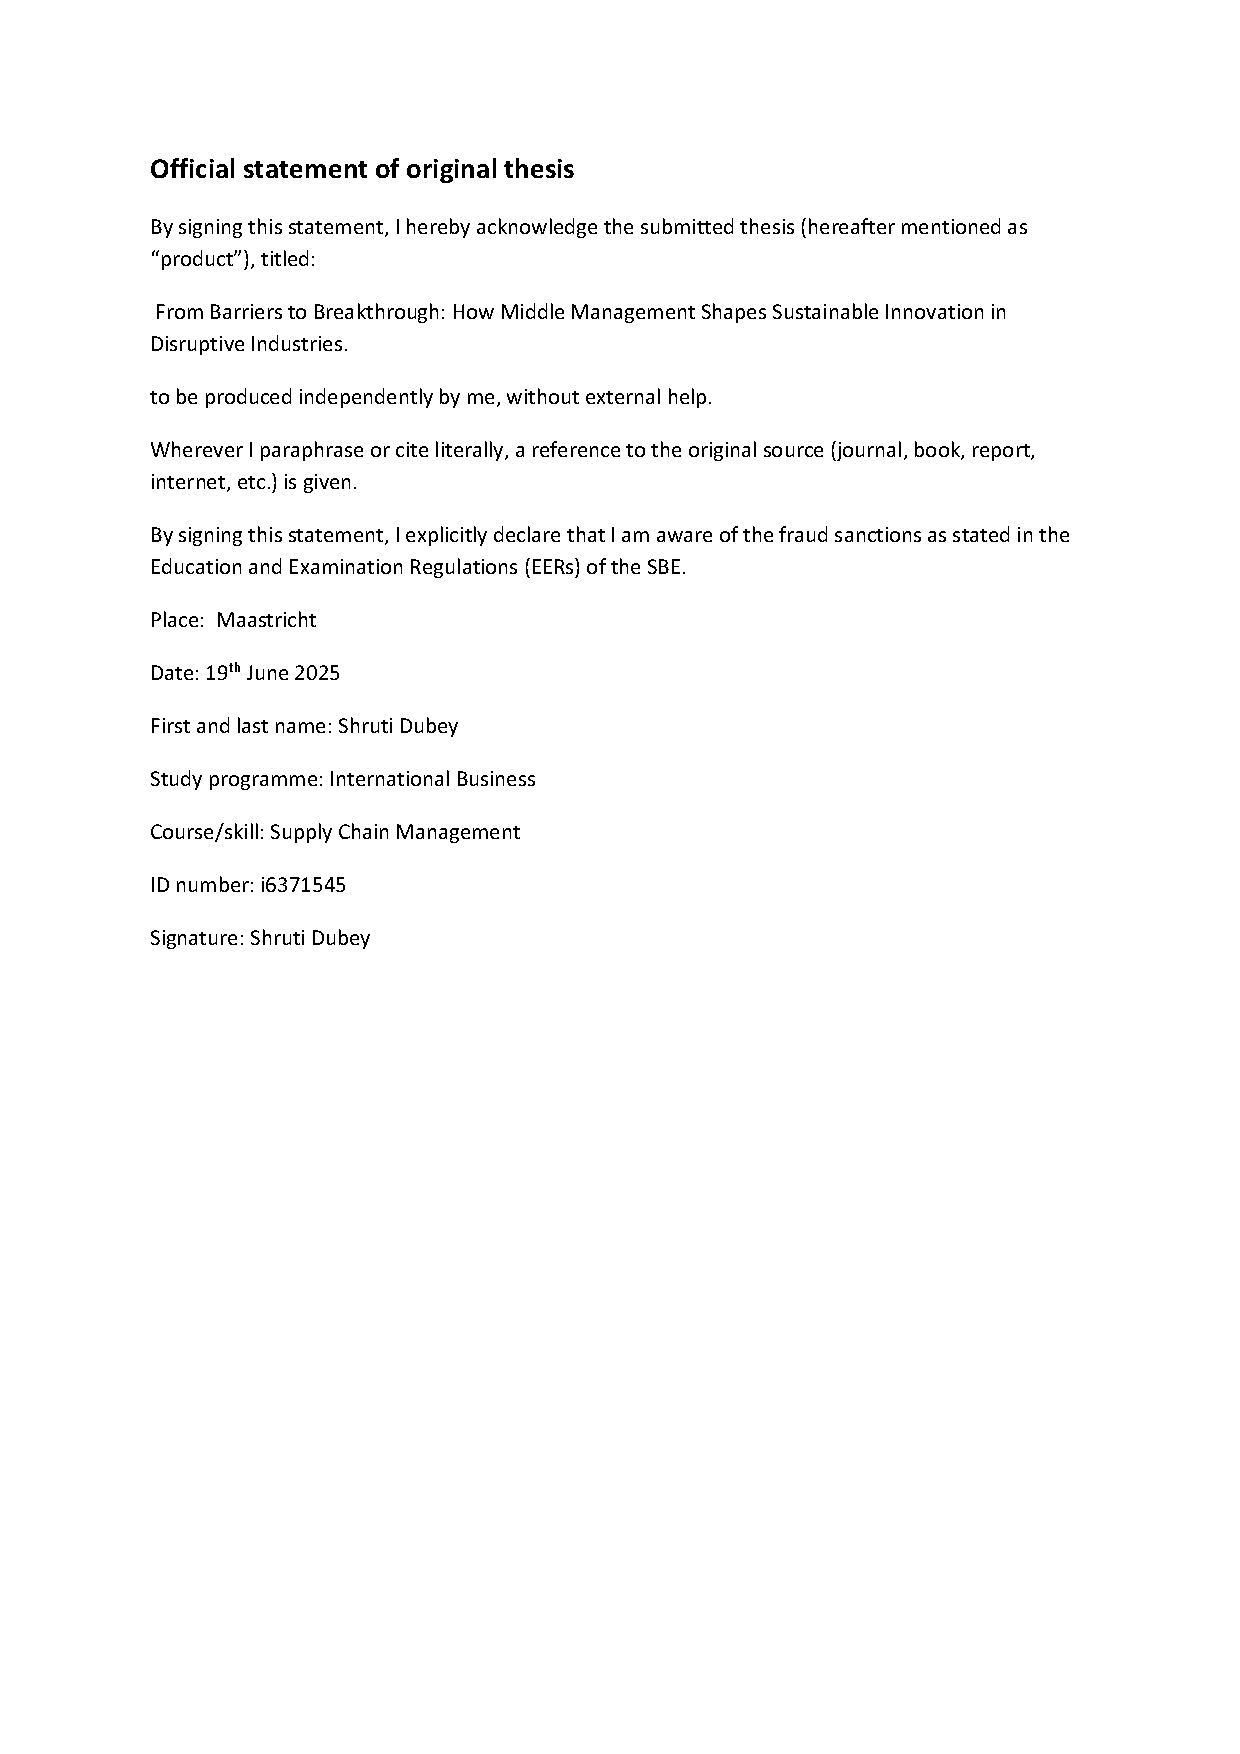
\includepdf[pages=-]{Images/original_thesis.pdf}
	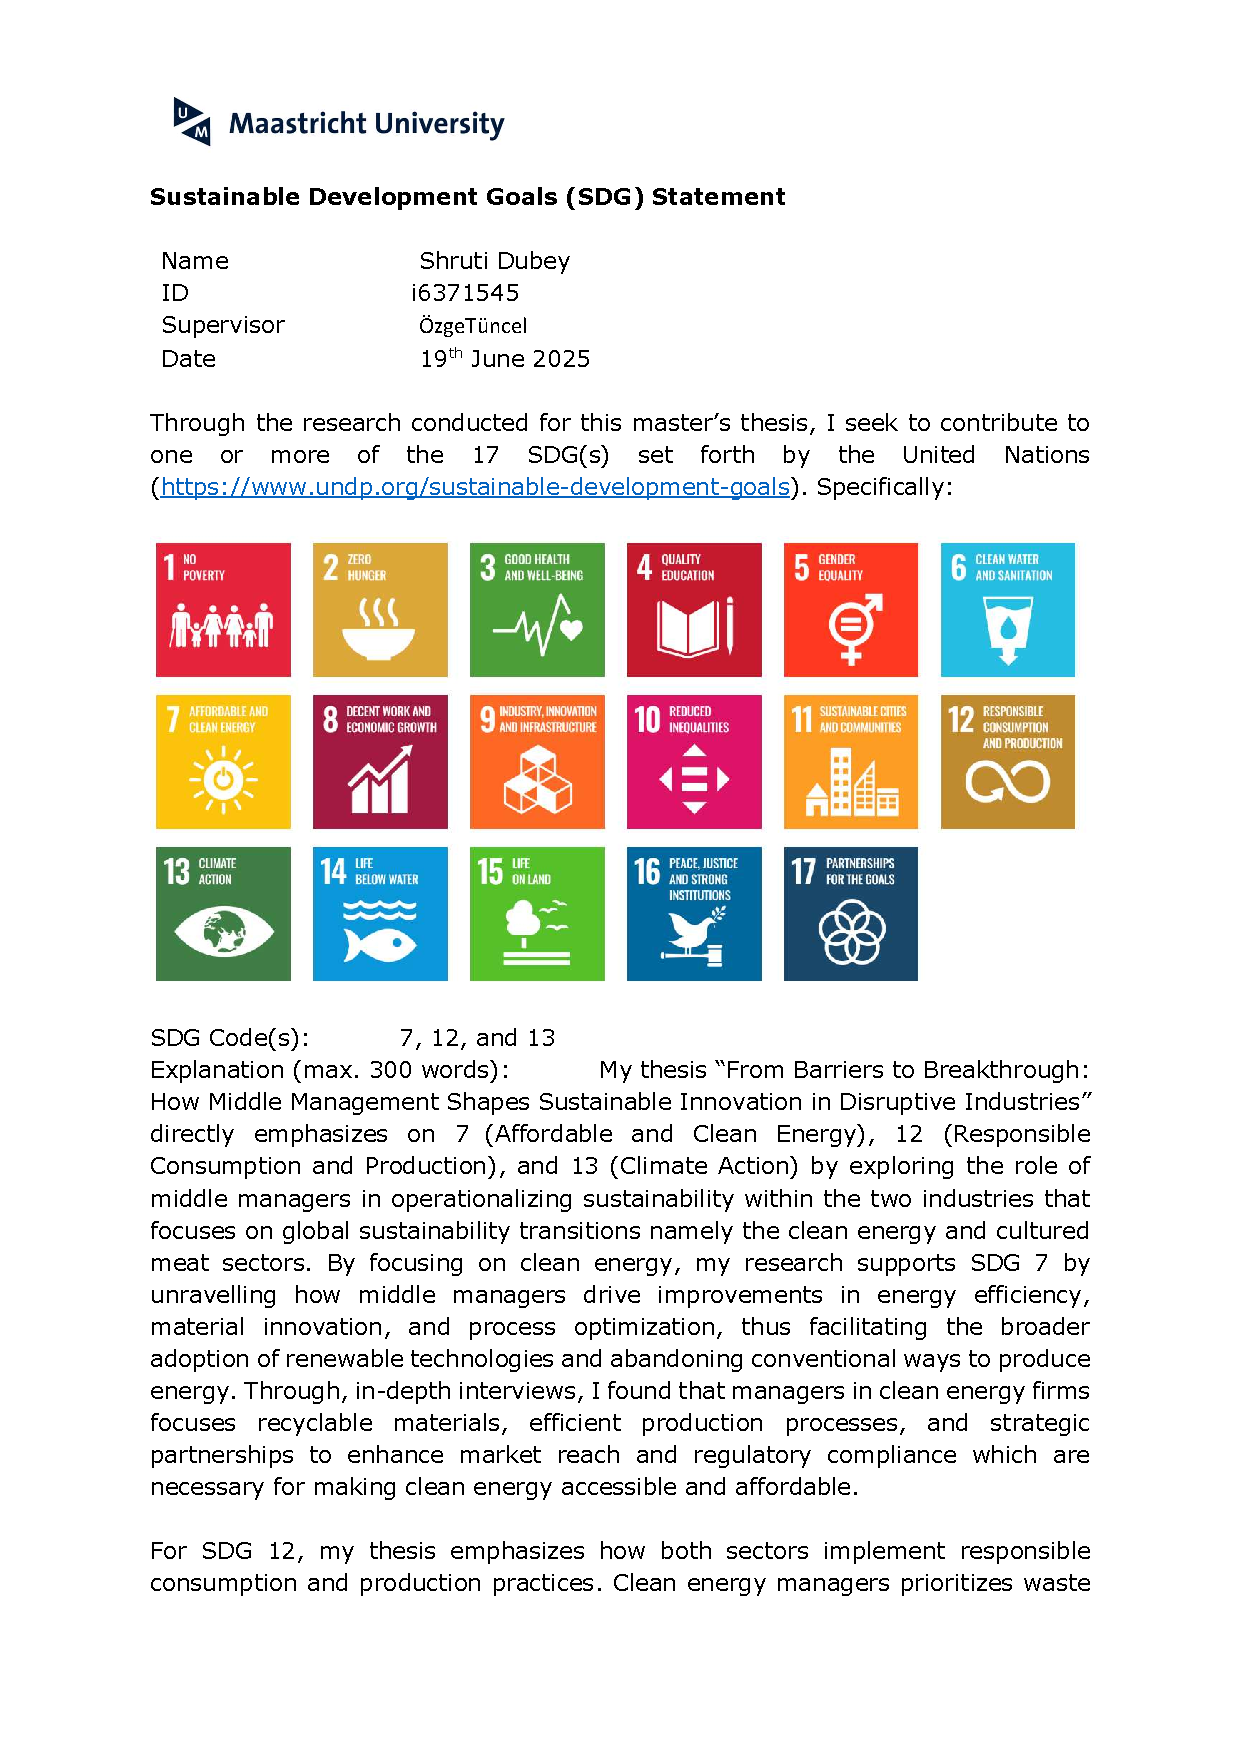
\includepdf[pages=-]{Images/SDG_Statement.pdf}
	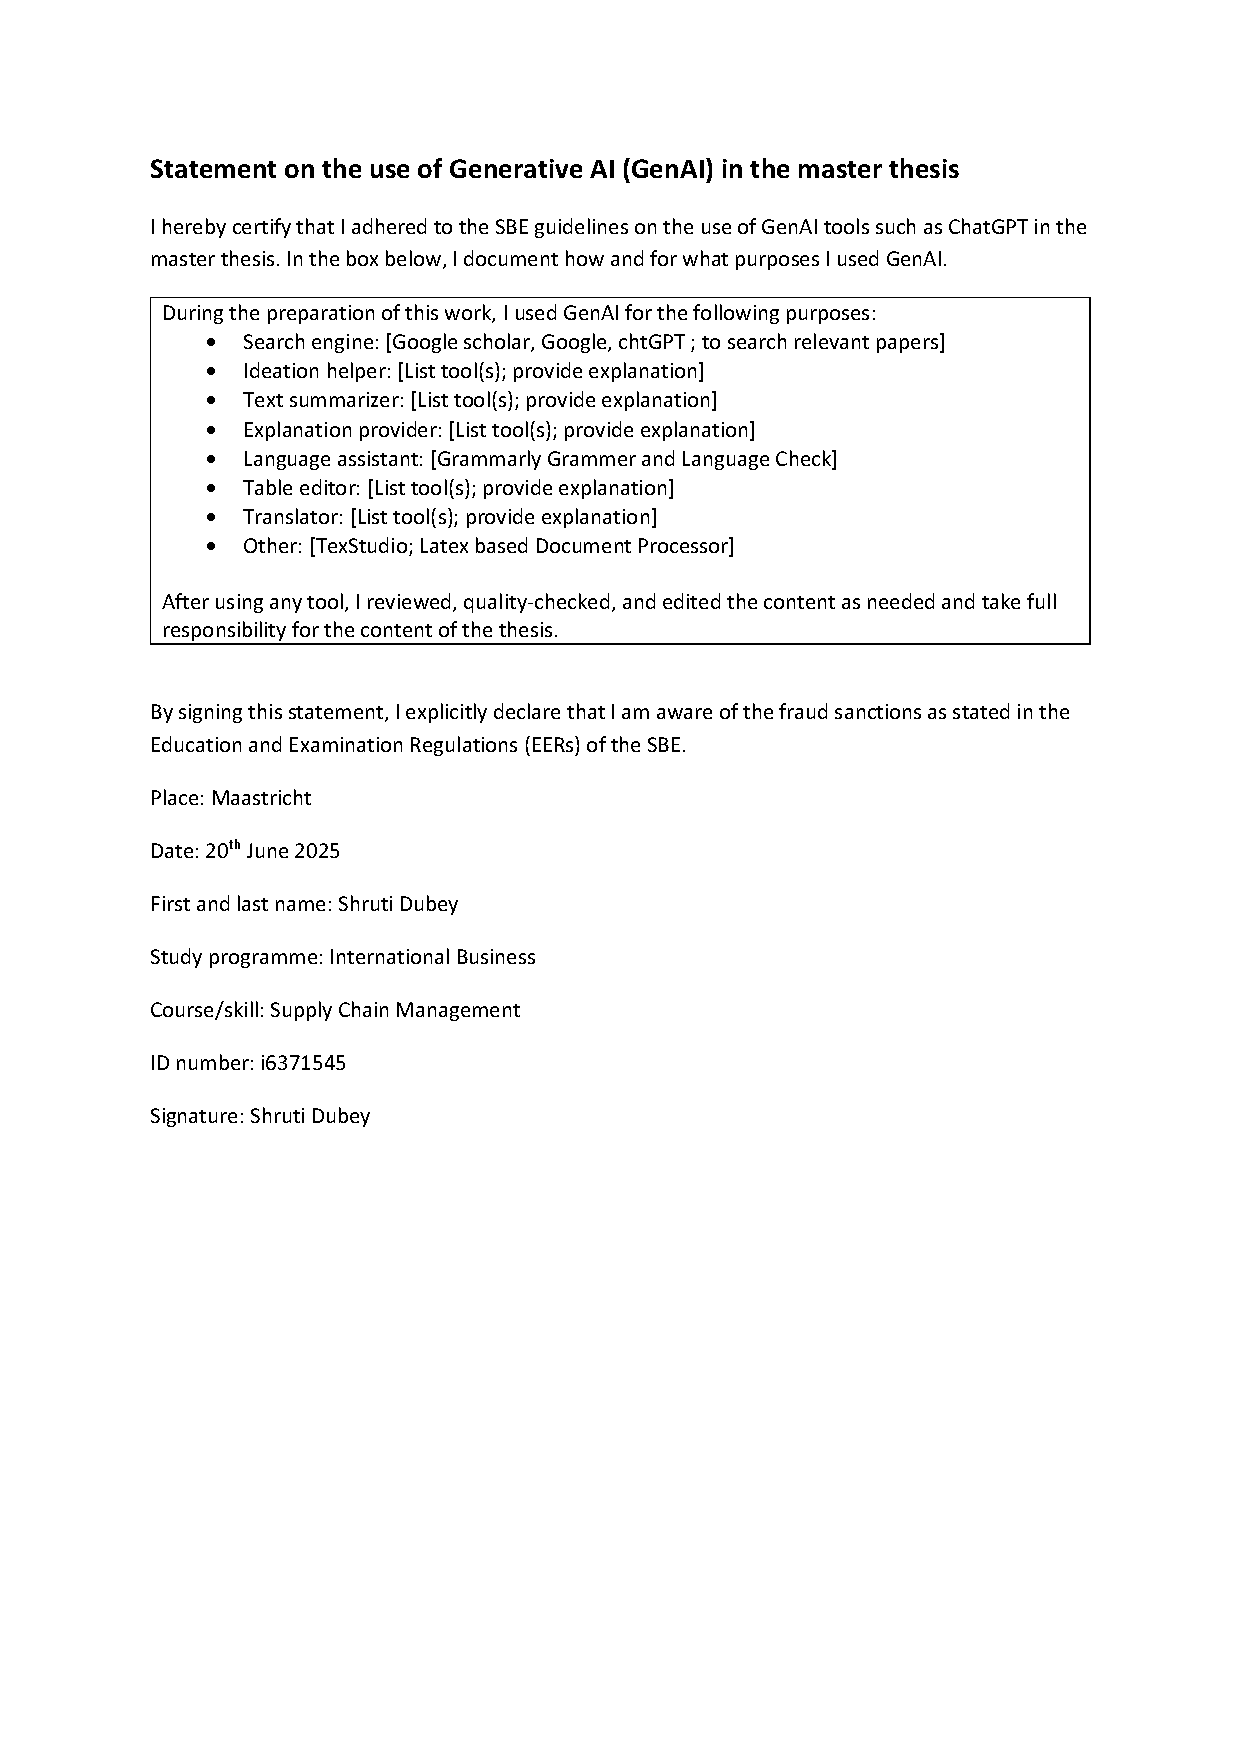
\includepdf[pages=-]{Images/GenAI.pdf}
	
\end{document}